\documentclass{article}
\usepackage{ctex}
\usepackage{hyperref}
\usepackage{geometry}
\usepackage{amsmath}
\usepackage{caption}
\RequirePackage{longtable,multirow,array}
\RequirePackage{booktabs}
\usepackage{booktabs}
\usepackage{multicol}
\usepackage{longtable}
\usepackage{xurl}
\usepackage{booktabs}
\usepackage{algorithm}
\usepackage{algpseudocode}
\usepackage{enumitem}
\usepackage[style=ieee,sorting=nyt]{biblatex}
\DefineBibliographyStrings{english}{
	references = {参考文献}
}
\assignrefcontextentries[]{*}
\addbibresource{References.bib}
\geometry{left=1in, right=1in, top=1in, bottom=1in}
\hypersetup{hidelinks}
\hypersetup{bookmarksnumbered=true,
	bookmarksopen=true,
	colorlinks=true,
	linkcolor=black,
	citecolor=blue,
	urlcolor=black}
\usepackage{tikz}
\usepackage{pgfplotstable}
\usepackage{pgfplots}
\pgfplotsset{compat=1.18}
\captionsetup{justification=centering}
\captionsetup[figure]{name={图},labelsep=space,labelfont=bf}
\captionsetup[table]{name={表},labelsep=space,labelfont=bf}
\CTEXoptions[today=old, contentsname=Contents]
\newcommand{\authyear}[1]{\citeauthor{#1} (\citeyear{#1})}
\setmainfont{Arial}

\newcommand{\toB}[1]{\color{blue}#1\color{black}}

\begin{document}
	\title{\vspace{-2.25cm} 眼科疾病诊断的多模态异常感知模型}
	\author{潘思齐}
	\date{}
	\maketitle
	
	\vspace{-0.2cm}
	\hrule
	\vspace{-0.1cm}
	\section*{摘要}
	\hrule
	\vspace{0.4cm}
	我们设计了一种新颖的模型,即多模态异常感知模型(MAAM),用于辅助眼科疾病的诊断。该模型允许输入两类眼科图像,分别是光学相干断层扫描(OCT)图像和彩色眼底图像,并基于异常来推导疾病,模拟眼科医生的决策过程。该模型由两个子模型组成,分别是异常模型和诊断模型。异常模型识别11种OCT异常和8种眼底异常;诊断模型通过整合异常模型的特征识别出12种疾病。在MAAM中,我们引入了融合机制、共显异常和疾病的概念、以及异常-疾病推导标准。该模型打破了复杂神经网络的“黑箱”,为眼科医生提供了更具可解释性的信息以供参考。模型的总体准确率为89\%,验证了其可行性。
	
	
	\vspace{0.4cm}
	\hrule
	\vspace{1cm}
	
	\begin{multicols}{2}
	
	\section{背景}
	
	眼科疾病可以通过多种方法诊断,包括使用光学相干断层扫描(OCT)和彩色眼底图像。眼科医生通常通过识别眼部异常来推导疾病。传统上,诊断主要依赖于眼科医生的专业经验和知识,这可能导致高误诊率和医疗数据的利用不足。随着人工智能(AI)的广泛应用,深度学习(DL)共享专家知识,为偏远地区的患者提供支持方面做出了巨大贡献 \autocite{Ichhpujani_Thakur_2021}。通过利用深度学习,研究人员开发了辅助诊断程序,以帮助眼科医生进行诊断。许多研究都使用卷积神经网络(CNN)来分析眼科图像。一些常用的 CNN 包括 VGG、ResNet 和 Inception \autocite{daich2023artificial}。在图像分割和寻找异常中,U-net 被广泛应用 \autocite{Ronneberger_Fischer_Brox_2015}。大多数研究在训练CNN时使用迁移学习,包括三个步骤:学习、微调和验证。
	
	一些研究直接从OCT图像预测疾病。\citeauthor{li2019deep} 使用ResNet分析OCT图像,并区分脉络膜新生血管(CNV)、糖尿病性黄斑水肿(DME)、玻璃疣(Drusen)和健康人眼。此外,他们还进行了遮挡测试,以找出对于诊断最重要的区域 \autocite{li2019deep}。\citeauthor{yoo2021feasibility} 使用生成对抗网络(GAN)和Inception-v3,结合少量数据集,探讨了改善罕见眼科疾病OCT诊断的可行性 \autocite{yoo2021feasibility}。他们通过从健康OCT图像中生成眼科疾病的OCT图像来解决图像数量不足和数据不平衡的问题。\citeauthor{Kermany2018} 通过基于图像的深度学习进行医学诊断,并识别可治疗的疾病。他们还提供了一个广为使用的数据库,其中包含超过十万张用于三种疾病的OCT的有标注图像 \autocite{Kermany2018}。
	
	其他研究可以从带注释的OCT图像中识别眼科异常。\citeauthor{camino2018deep} 利用深度学习在面部OCT中识别未凋亡的的光感受器区域,用于脉络膜疾病和视网膜色素变性(RP) \autocite{camino2018deep}。\citeauthor{srinivasan2014fully} 通过展平图像,使用支持向量机(SVM)提取视网膜层的厚度信息,检测 DME 和干性年龄相关性黄斑变性(干性AMD) \autocite{srinivasan2014fully}。\citeauthor{leandro2023oct} 使用VGG,用中央黄斑横截面OCT检测多达8种关键异常并由此检测多种疾病 \autocite{leandro2023oct}。\citeauthor{Fang_Wang2019} 开发了一种新的病灶感知 CNN,称为 LACNN,用于模拟集中于眼科异常的眼科医生诊断 \autocite{Fang_Wang2019}。
	
	另一些研究使用眼底图像来预测眼科疾病。\citeauthor{masumoto2019accuracy} 使用超宽视野眼底图像训练深度 CNN 以诊断 RP \autocite{masumoto2019accuracy}。\citeauthor{chen2021artificial} 使用彩色眼底照片和多种 CNN(如 Inception V3、Inception Resnet V2 和 Xception),开发了 RP 的早期检测方法 \autocite{chen2021artificial}。\citeauthor{li2022development} 使用 CNN 基于彩色眼底摄影检测多达 12 种眼底疾病 \autocite{li2022development}。\citeauthor{Son2023} 提出了一种新颖的架构和算法设计,从黄斑中心的眼底图像中综合识别 15 种异常和诊断 8 种主要眼科疾病。他们定义了反事实归因比(CAR)的概念,以解释系统的诊断原因,并揭示异常与疾病之间的关系 \autocite{Son2023}。
	
	近年来,越来越多的深度学习系统开始使用多模态信息来预测眼科疾病。对于自动化检测系统,从 OCT 图像和眼底图像中提取特征可以有效避免诊断偏差和不完整性。虽然并不总是能带来更好的自动诊断结果,但它确实有助于眼科医生做出更准确和全面的临床决策。例如,\citeauthor{liu2023prediction} 结合 OCT 和眼底图像,评估视网膜色素变性患者的视力损害 \autocite{liu2023prediction}。\citeauthor{Xu2021} 利用双模态 CNN 诊断 AMD 和脉络膜息肉样血管病变(PCV),其中架构使用眼底和 OCT 图像作为迁移学习 CNN 的输入,并将提取的特征拼接以分类干性 AMD、湿性 AMD 和 PCV 三种疾病 \autocite{Xu2021}。\citeauthor{Andrearczyk2018} 将医学图像与生物医学文本信息结合起来,以区分不同的疾病,这是多模态应用的一种创新方法 \autocite{Andrearczyk2018}。
	
	多模态诊断的关键技术问题在于如何融合来自多种来源的结果。融合有三种类型,即早期融合、后期融合和混合融合。决定最佳融合类型是应用深度学习方法探索过程的一部分 \autocite{Ichhpujani_Thakur_2021}。
	
	\section{概述}
	\label{sec:overview}
	
	我们开发了多模态异常感知模型(MAAM)来协助眼科医生诊断眼科疾病。该模型同时考虑 OCT 和彩色眼底图像输入。此外,它模拟了眼科医生在检查患者时的决策过程,即首先识别异常,然后推导疾病。该模型设计部分打开了深度学习的“黑箱”,并为眼科医生提供了更多可解释的信息参考。
	
	MAAM 的结构如图~\ref{fig:3_parts} 所示。模型由两个子模型组成:异常模型和诊断模型。我们将多个 OCT 和眼底图像输入到异常模型中,并将异常分类结果作为诊断模型的输入,诊断模型最终输出疾病概率。
	
	\vspace{0.5cm}
	
	异常模型实际上是异常分类器,即图像中可直接观察到的症状。MAAM 能识别 11 种 OCT 异常和 8 种眼底异常,如图~\ref{fig:OCT_abnormities} 和图~\ref{fig:fundus_abnormities} 所示。“附录”中列出了异常和疾病的缩写及详细信息。
	
	异常模型还包括两个子模型:OCT 模型和眼底模型,分别对 OCT 和眼底异常进行分类。两个子模型都使用 CNN,并修改了最终的全连接层(FC 层)。我们比较了四种常用 CNN 的性能:ResNet152、ResNet50、ResNet18 \autocite{He_Zhang_Ren_Sun_2016}和 VGG16 \autocite{Simonyan_Zisserman_2015},并为每个子模型选择了最佳模型。每个 CNN 的最终 FC 层被修改,使其输出向量的大小等于 OCT 或眼底异常的数量。为了对输出向量进行归一化,我们对其进行了 softmax 操作。每个子模型输出所有异常的概率向量。
	
	\vspace{0.5cm}
	
	诊断模型包括两个阶段:阶段 D1 和阶段 D2。
	
	\vspace{0.2cm}
	
	在阶段 D1 中,我们根据异常模型的概率向量确定每种疾病的严重程度。我们使用异常-疾病推导标准(见图~\ref{fig:criteria})作为判断依据。阶段 D1 中有多个子模型,每个子模型对应一种疾病。根据推导标准,我们确定一种疾病的异常数量,并以此来定义严重程度。例如,疾病“rDR”中共有 5 种异常:OCT 异常“DME”以及眼底异常“HM”、“VA”、“MA”和“CWP”。因此,考虑到健康状态,我们将“rDR”定义为 6 个严重程度级别。
	
	我们使用融合后的向量作为阶段 D1 中每个子模型的输入,让向量通过一个 FC 层和 softmax 操作,以生成严重程度的概率向量。
	
	在阶段 D2 中,我们确定最终的疾病概率向量。同样,我们使用阶段 D1 中子模型的输出,进行向量融合,通过 FC 层并进行 softmax 操作,输出潜在疾病的概率,供眼科医生参考。
	
	\end{multicols}
	
	\begin{figure}[htbp]
		\centering
		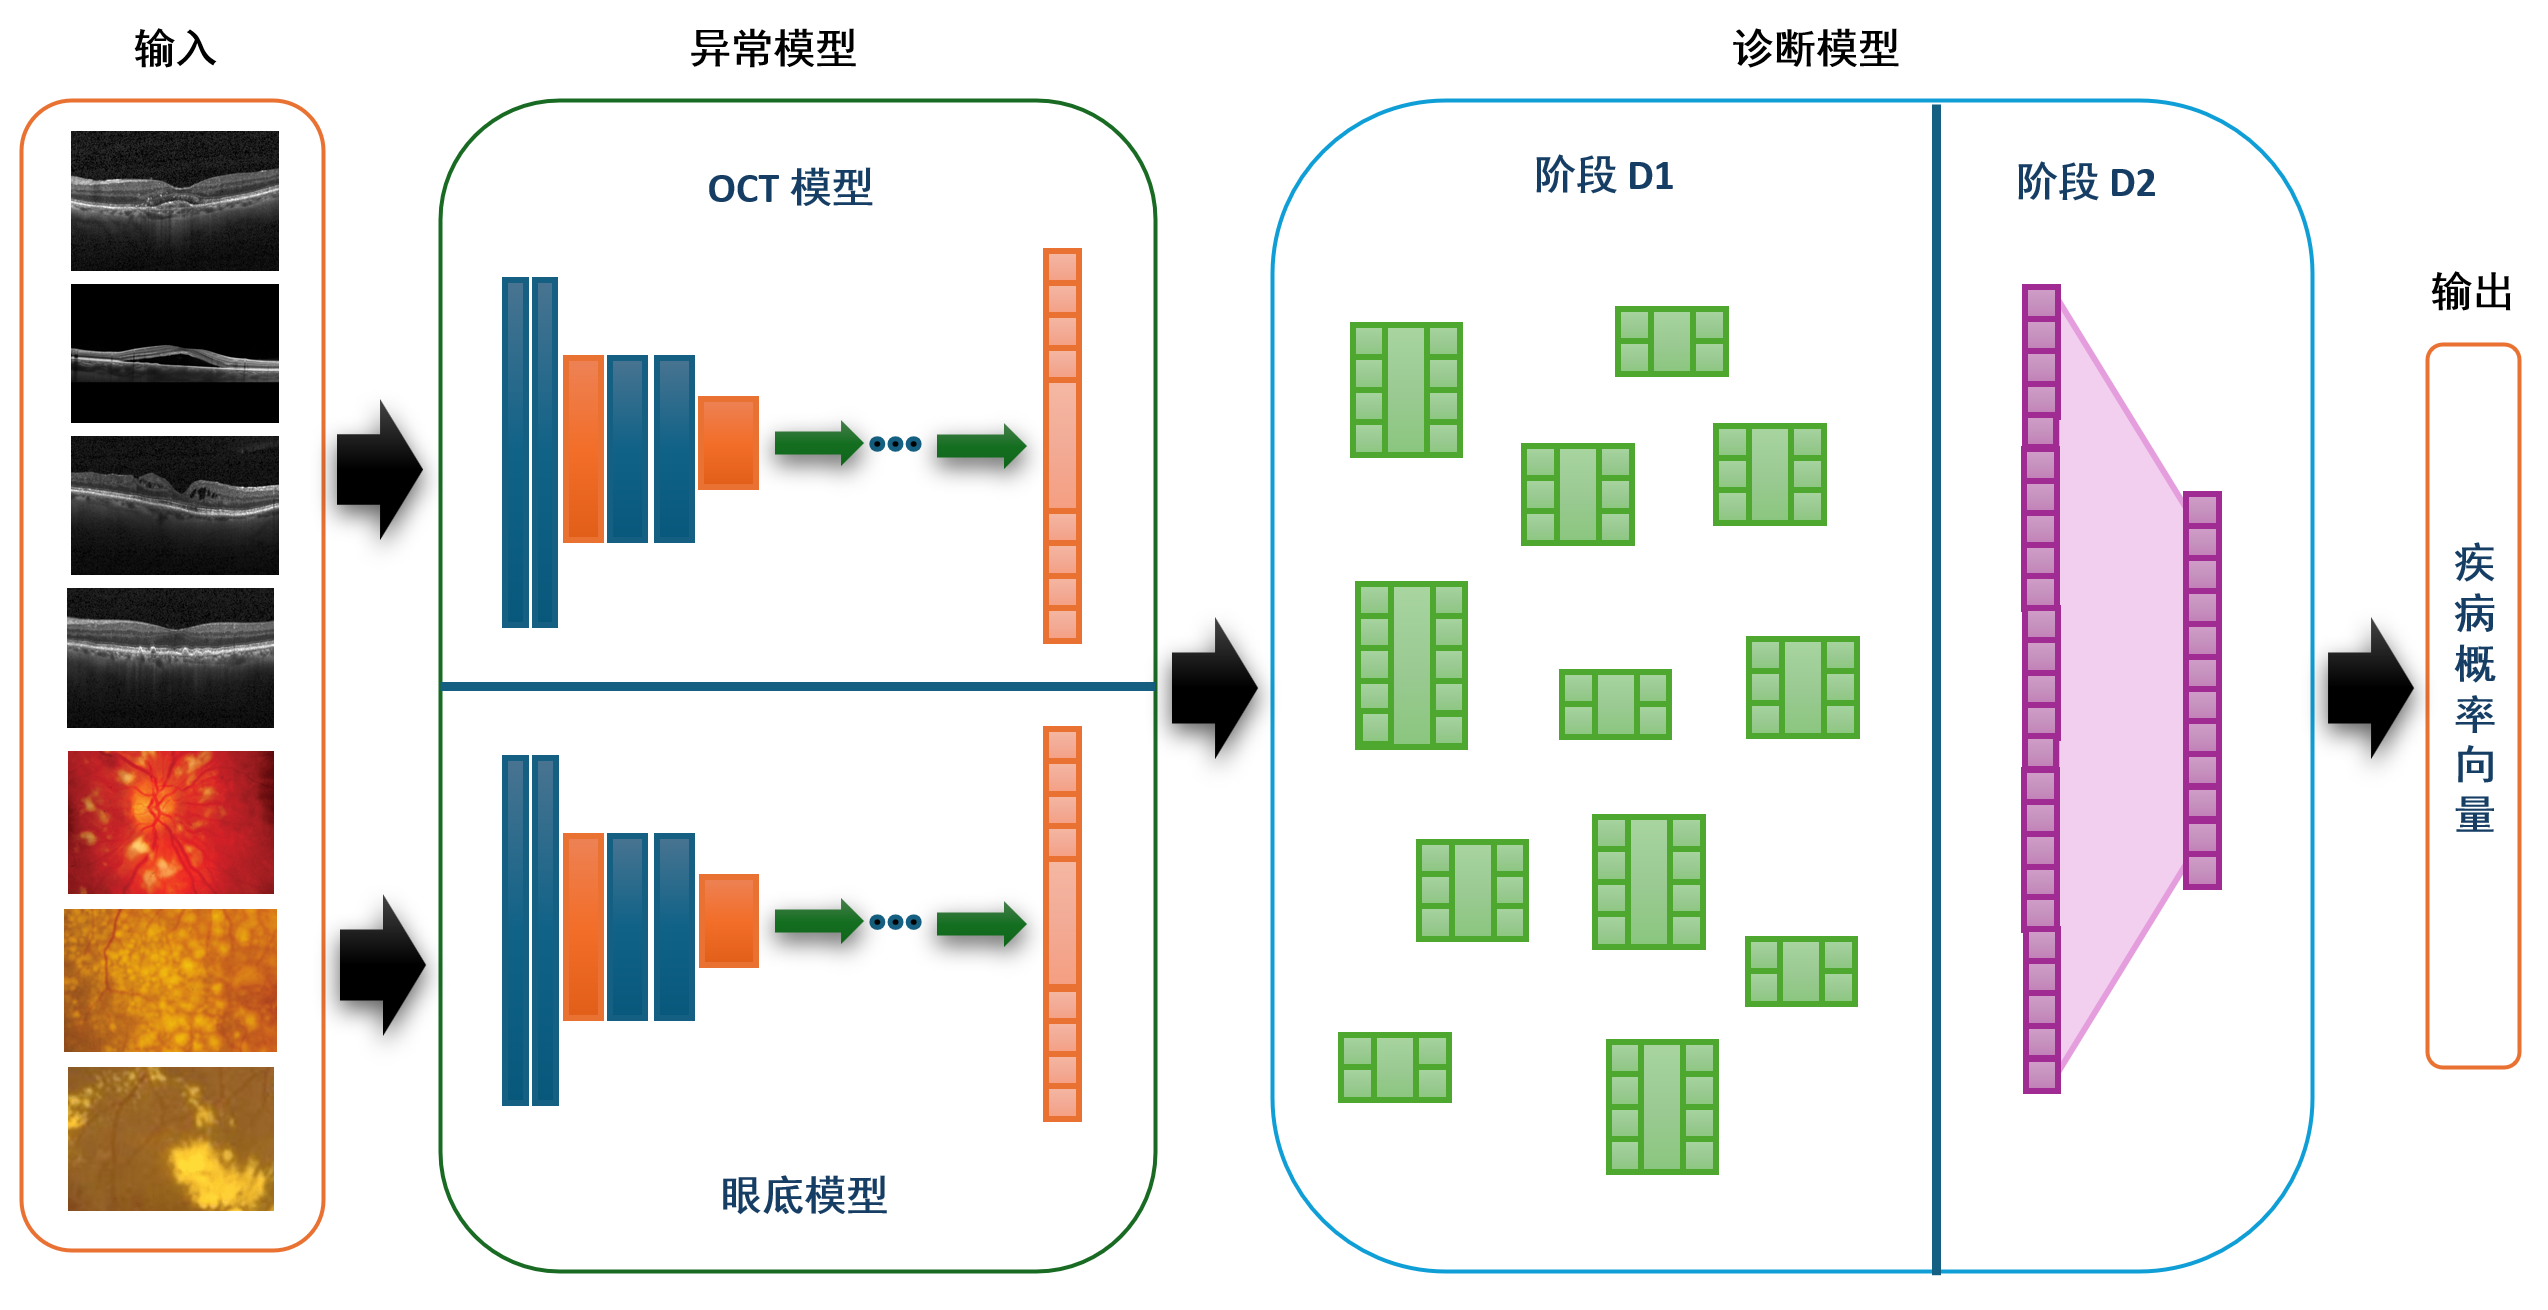
\includegraphics[width=\linewidth]{Figs/model_overview.png}
		\caption{模型总览}
		\vspace{0.3cm}
		\label{fig:3_parts}
		\vspace{1cm}
	\end{figure}
	
	\begin{multicols}{2}
	
	在 MAAM 中,我们利用融合操作整合不同子模型的结果。如图~\ref{fig:fusion} 所示,MAAM 中总共有三次融合操作。
	
	第一次融合发生在 OCT 模型或眼底模型的输出中。在实际场景中,可以使用多个 OCT 和眼底图像进行眼科疾病诊断。每张图像通过 OCT 或眼底模型后得到一个概率向量。为了利用所有图像的概率结果,我们对所有向量进行了最大化融合,从而得到一个 OCT 异常概率向量和一个眼底异常概率向量,均取最大值。
	
	第二次融合发生在异常模型与阶段 D1 之间的接口。我们将 OCT 异常概率向量和眼底异常概率向量进行拼接融合,作为阶段 D1 所有子模型的输入。
	
	第三次融合发生在阶段 D1 与阶段 D2 之间的接口。我们将所有严重程度向量进行拼接,输入阶段 D2 模型。融合向量通过 FC 层并经过 softmax 操作,输出最终结果。
	
	\section{异常模型}
	
	\subsection{数据准备}
	
	用于训练的图像和标签主要从公共数据库中下载,但部分异常不包含在这些数据库中。对于这些异常,我们使用搜索引擎作为额外的数据来源获取图像。各数据来源获得的图像数量如表~\ref{tb:OCT_source} 和表~\ref{tb:Fundus_source} 所示。图像的搜索引擎链接详见“附录”。
	
	对于图像少于 1000 张的 OCT 异常,我们使用 Cycle-GAN \autocite{Zhu_Park_Isola_Efros_2020}生成新图像。我们训练一个 Cycle-GAN 网络,将健康图像与异常图像进行转换,取出将健康图像转换为异常图像的生成器,用其生成新的异常图像。我们检查所有生成的图像,选取那些清晰显示了目标异常的图像。采纳率见表~\ref{tb:cycleGAN_number}。由于生成的眼底图像过于模糊,眼底异常通常不如 OCT 明显,Cycle-GAN 无法从少量眼底图像中学习,因此我们不使用 Cycle-GAN 生成眼底图像。
	
	\end{multicols}
	
	\begin{figure}[htbp]
		\centering
		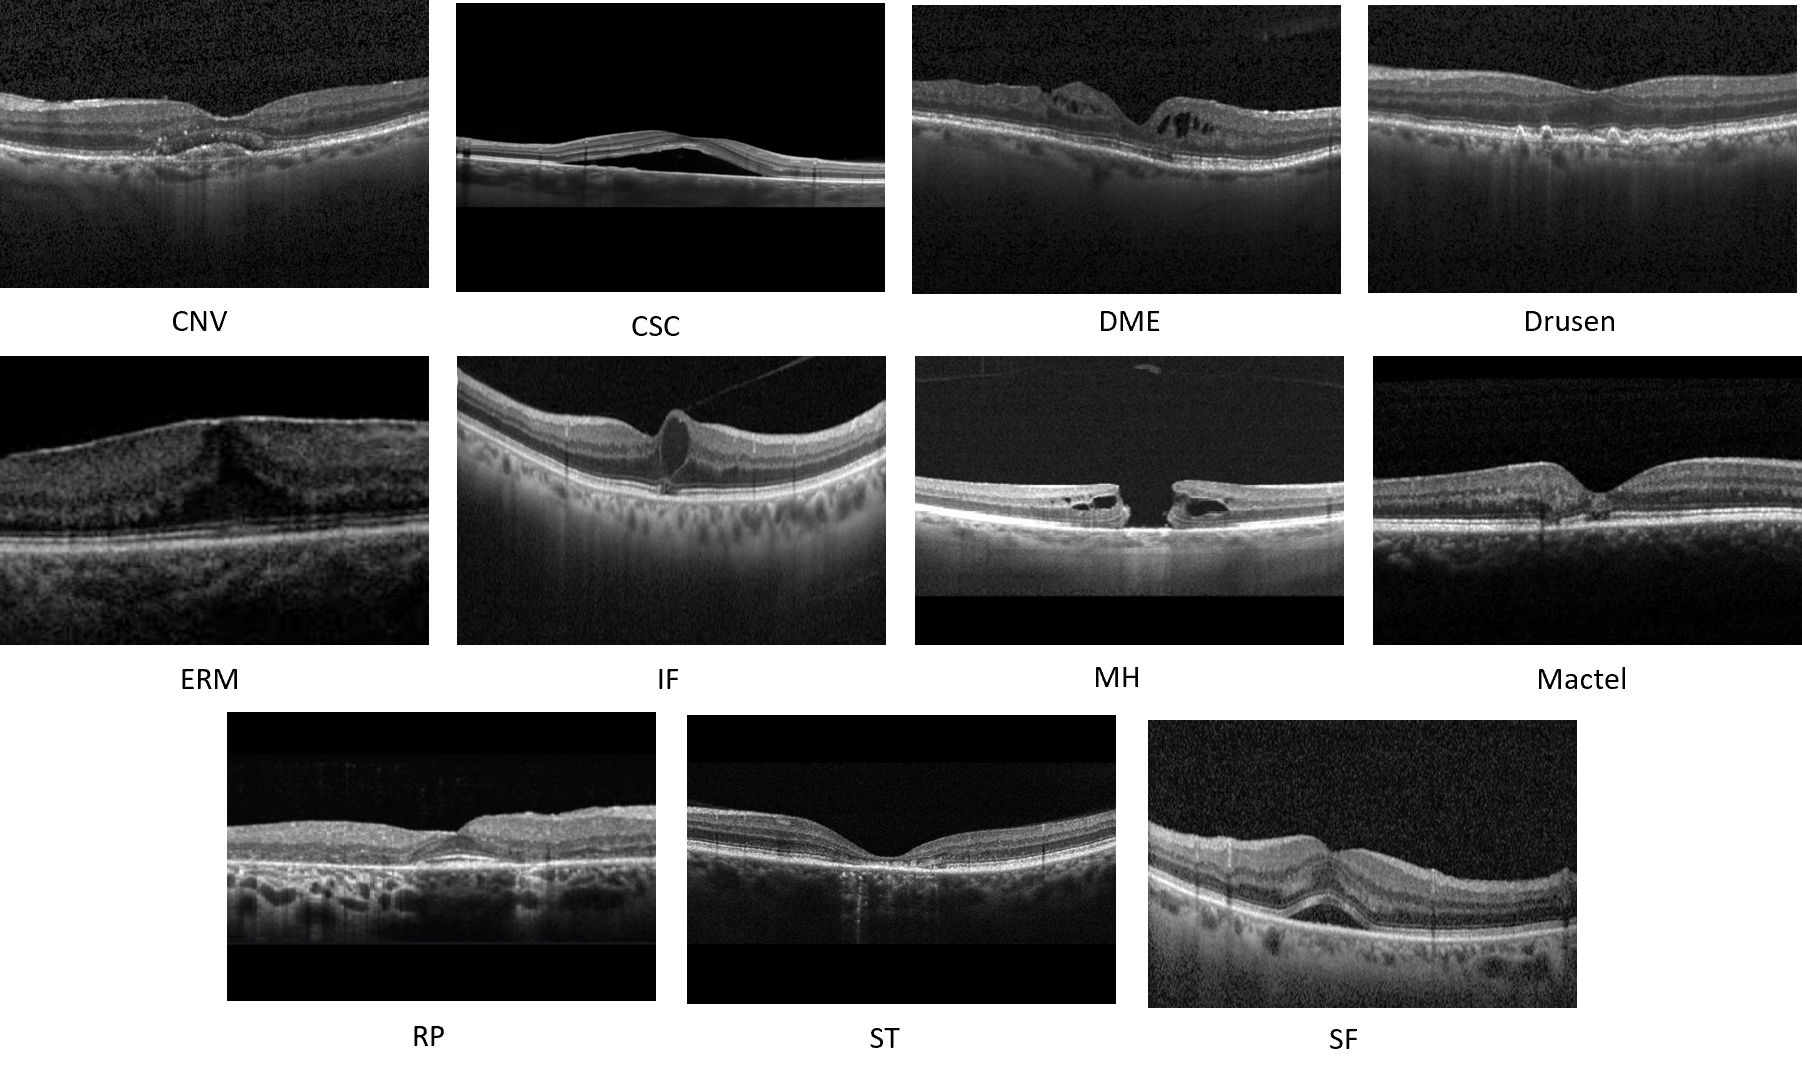
\includegraphics[width=\linewidth]{Figs/OCT_Abnormities.png}
		\caption{OCT异常 \autocite{Duker_Waheed_Goldman_2022}}
		\vspace{0.3cm}
		\label{fig:OCT_abnormities}
	\end{figure}
	
	\begin{figure}[htbp]
		\centering
		\includegraphics[width=\linewidth]{Figs/fundus_Abnormities.png}
		\caption{眼底异常 \autocite{Wolf_Kirchhof_Reim_2006}}
		\vspace{0.3cm}
		\label{fig:fundus_abnormities}
	\end{figure}
	
	\begin{figure}[htbp]
		\centering
		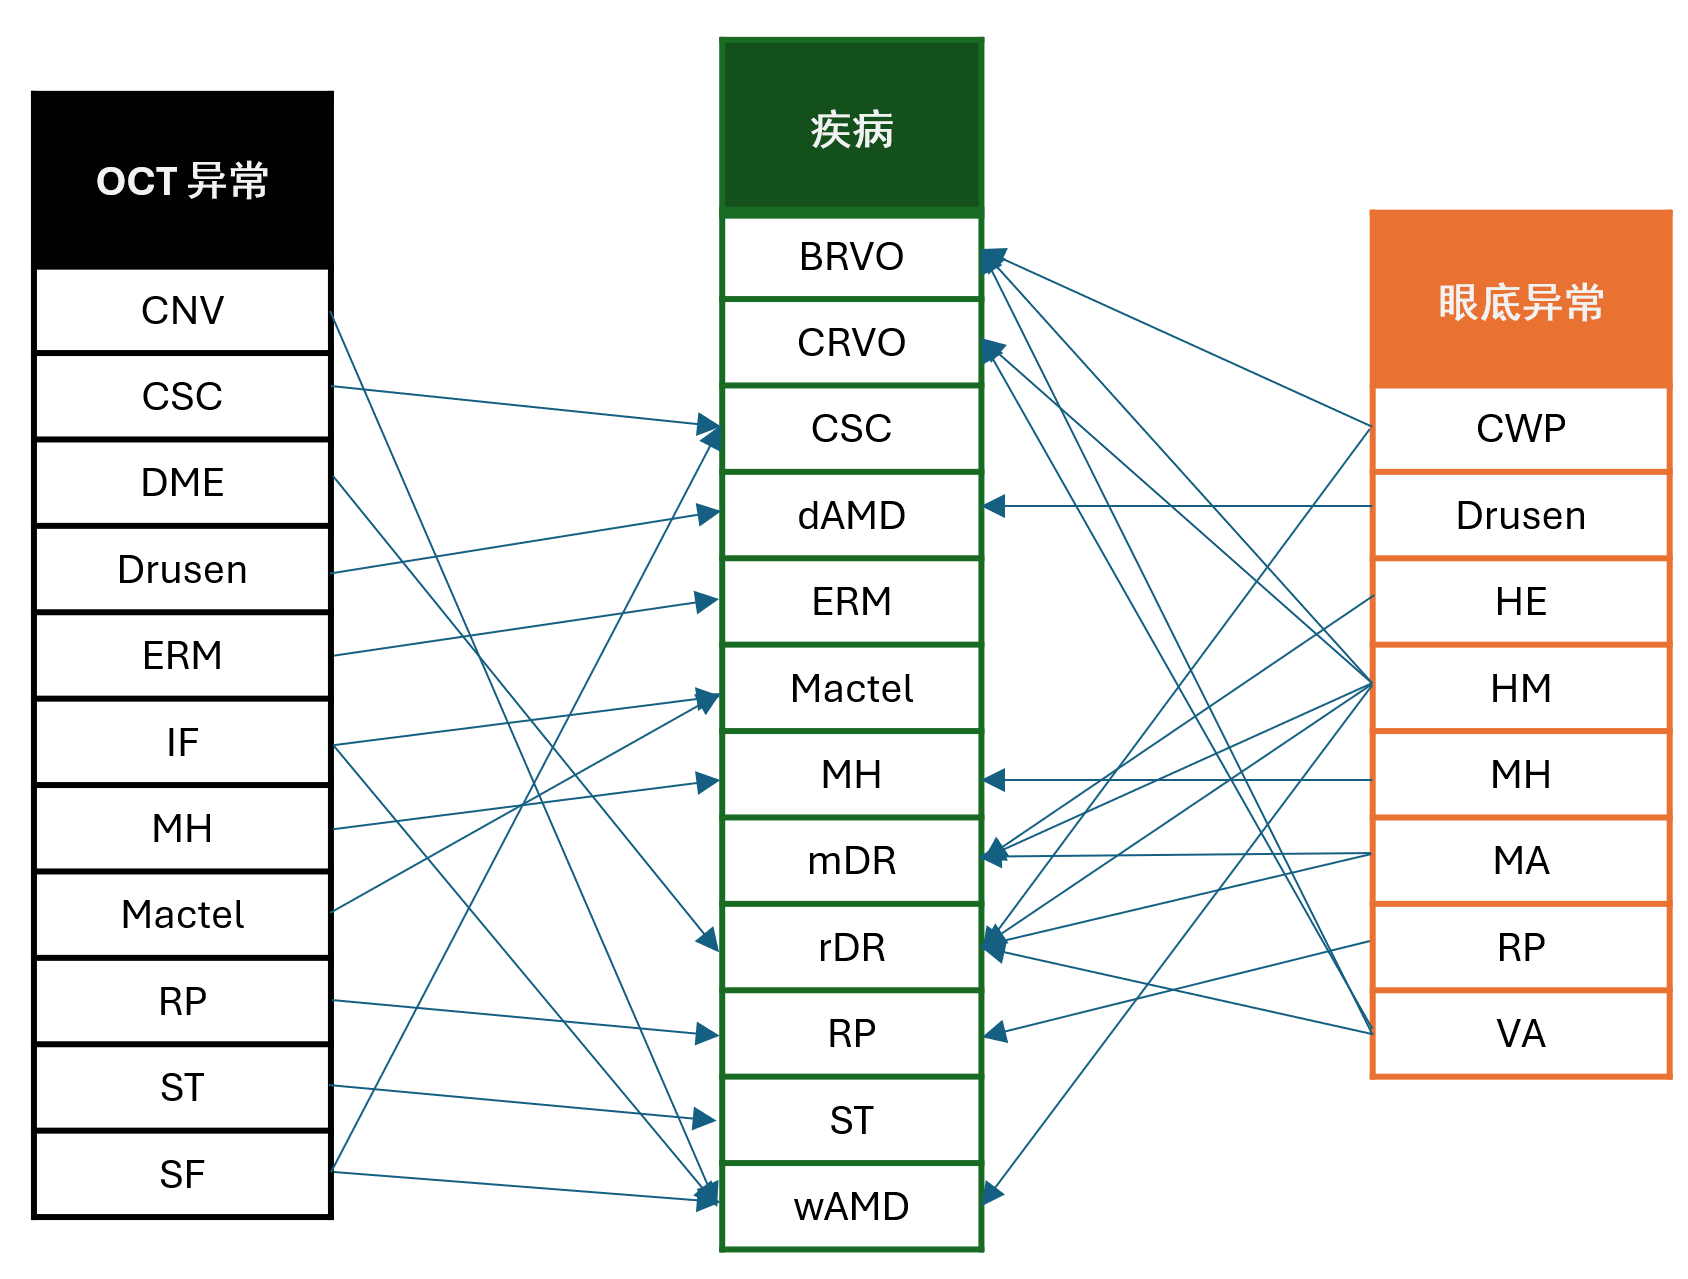
\includegraphics[width=0.7\linewidth]{Figs/criteria.png}
		\caption{异常-疾病推导标准}
		\vspace{0.3cm}
		\label{fig:criteria}
	\end{figure}

	\vspace{0.2cm}

	\begin{figure}[htbp]
	\centering
	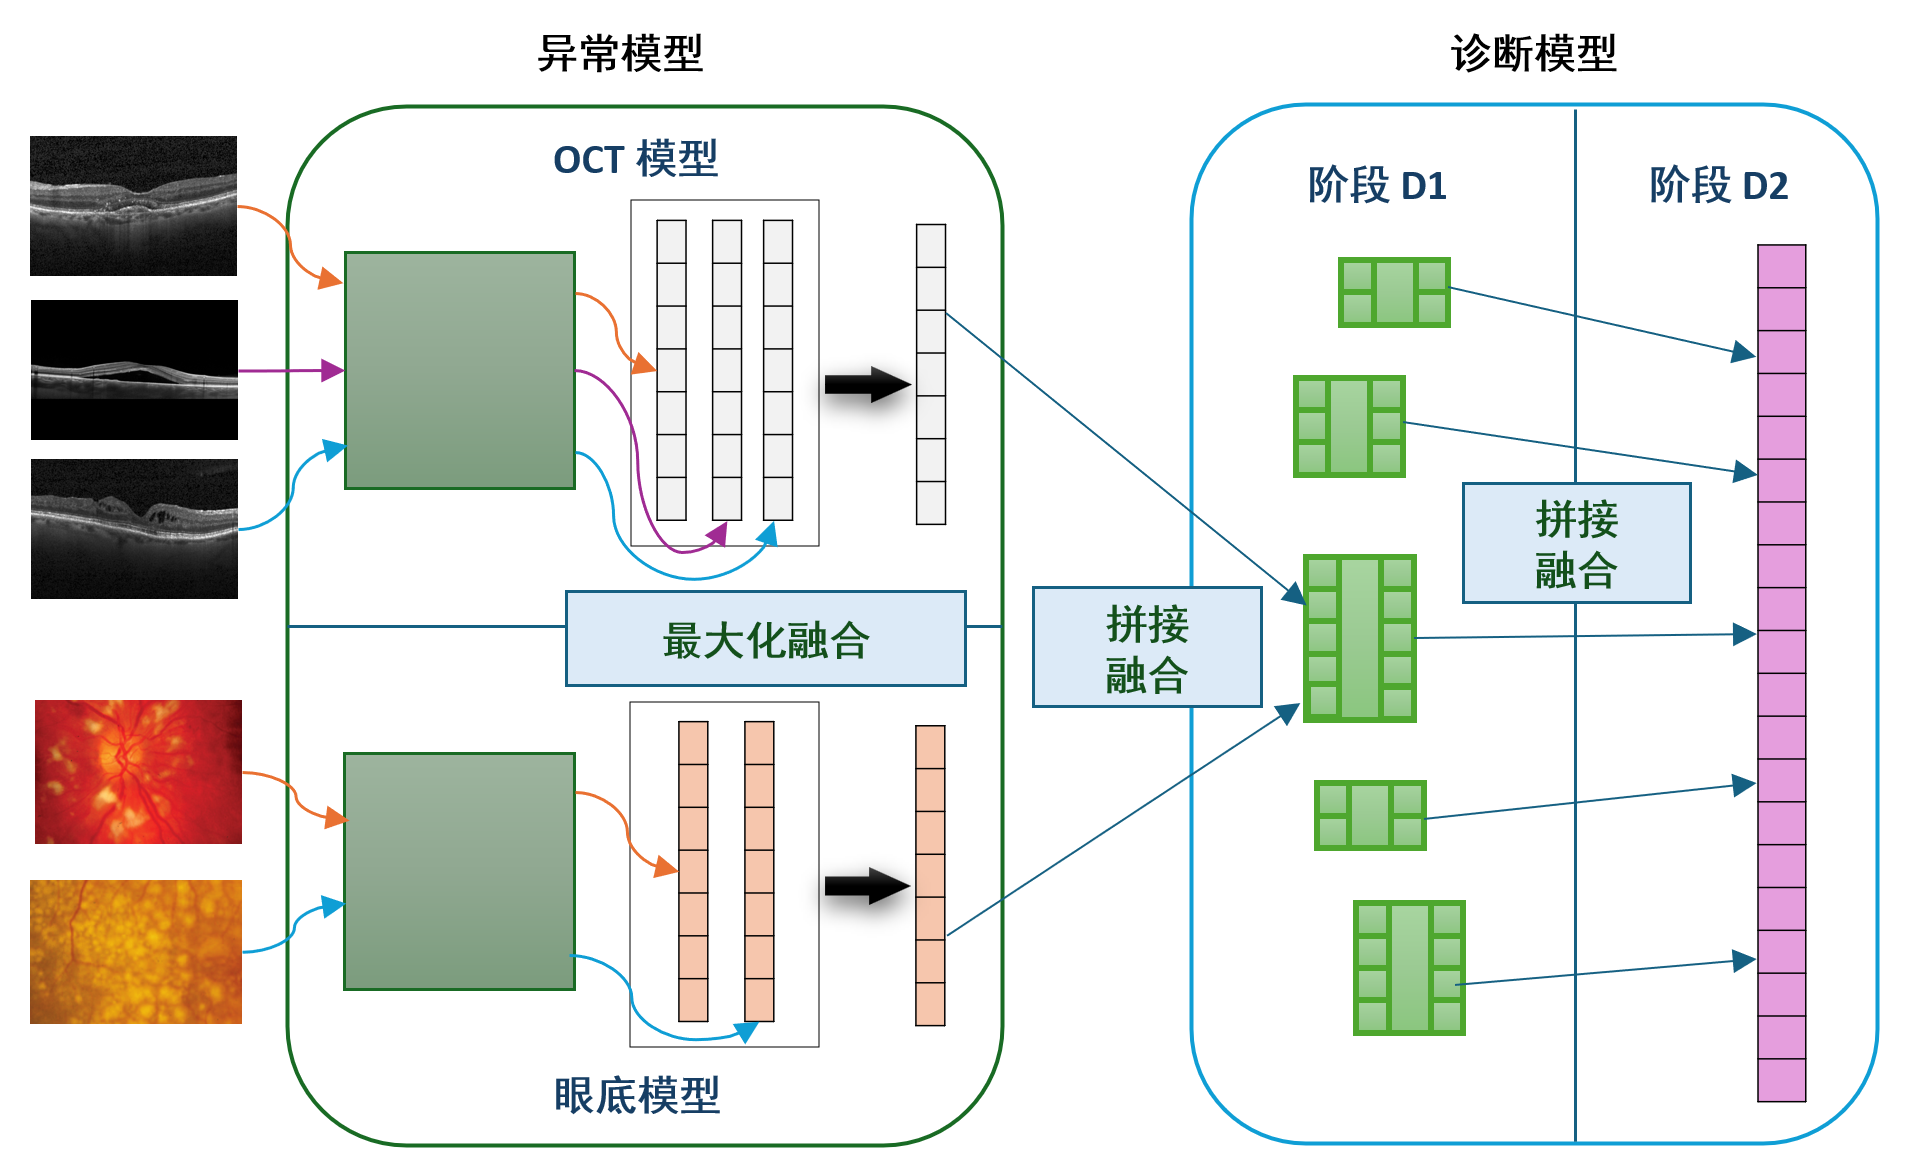
\includegraphics[width=\linewidth]{Figs/fusion.png}
	\caption{融合机制}
	\vspace{0.3cm}
	\label{fig:fusion}
	\end{figure}
	
	\pagebreak
	
	\begin{multicols}{2}
	我们将包括生成图像在内的图像分成训练和测试数据集,并对图像进行一系列变换,包括水平翻转、亮度随机变化(-10\% 到 +10\%)、水平和垂直随机平移(-5\% 到 +5\%)、随机缩放(-20\% 到 +20\%)和随机旋转(OCT 图像为 -10° 到 +10°,眼底图像为 -30° 到 +30°)。旋转仅应用于训练数据集中的图像。最终,我们为每个 OCT 异常获得 5000 张训练图像和 500 张测试图像,为每个眼底异常获得 3000 张训练图像和 300 张测试图像。
	\end{multicols}
		
	
		
		
		\vspace{-0.5cm}
		\begin{minipage}[t]{0.4\linewidth}
			{
				\fontsize{9}{12}\selectfont
				{
					\begin{longtable}{cccccc}
						\caption{OCT数据源}
						\label{tb:OCT_source}\\
						\toprule
						\multirow{2}{*}{异常}&\multicolumn{4}{c}{数据源}&\multirow{2}{*}{总数据量}\\
						&1&2&3&4&\\
						\midrule
						CNV    &2984&-  &- &- &2984\\
						CSC    &-   &102&32&- &134 \\
						DME    &2500&-  &- &- &2500\\
						Drusen &2500&-  &- &- &2500\\
						ERM    &-   &-  &- &16&16  \\
						IF     &1097&-  &- &- &1097\\
						MH     &-   &99 &31&- &130 \\
						Mactel &-   &-  &29&- &29  \\
						Healthy&5000&-  &- &- &5000\\
						RP     &-   &102&31&- &133 \\
						ST     &-   &-  &23&- &23  \\
						SF     &1083&-  &- &- &1083\\
						\bottomrule
					\end{longtable}
					
					\vspace{0.5cm}
					\begin{enumerate}
						\item Normal Disease Database \autocite{Kermany_database}
						\vspace{-0.2cm}
						
						\item OCTID \autocite{Gholami_Roy_Parthasarathy_Lakshminarayanan_2020}
						\vspace{-0.2cm}
						
						\item Few-shot \autocite{Yoo_2020}
						\vspace{-0.2cm}
						
						\item 搜索引擎
						\vspace{-0.2cm}
					\end{enumerate}
					
					\vspace{0.5cm}
				}
			}
		\end{minipage}
		\begin{minipage}[t]{0.6\linewidth}
			{
				\fontsize{9}{12}\selectfont
				{
					\begin{longtable}{cccccccc}
						\caption{眼底数据源}
						\label{tb:Fundus_source}\\
						\toprule
						\multirow{2}{*}{异常}&\multicolumn{6}{c}{数据源}&\multirow{2}{*}{总数据量}\\
						&1&2&3&4&5&6&\\
						\midrule
						CWP    &-  &- &- &33 &205&- &238\\
						Drusen &-  &- &- &50 &-  &- &50 \\     
						HE     &20 &- &- &75 &284&- &379\\ 
						HM     &13 &66&- &105&278&- &462\\     
						MH     &-  &- &- &-  &-  &34&34 \\        
						MA     &55 &- &- &1  &219&- &275\\
						Healthy&100&37&15&-  &-  &- &152\\      
						RP     &-  &22&- &-  &-  &44&66 \\         
						VA     &-  &64&- &14 &-  &- &78 \\
						
						\bottomrule
					\end{longtable}
					
					\vspace{1cm}
					\begin{enumerate}[left=1.5cm]
						
						\item E-ophtha \autocite{E_ophtha}.
						\vspace{-0.2cm}
						
						\item Kaggle1000 \autocite{1000Fundus_Pytorch_TransferLearning}
						\vspace{-0.2cm}
						
						\item HRF \autocite{HRF_2013}
						\vspace{-0.2cm}
						
						\item STARE \autocite{STARE}
						\vspace{-0.2cm}
						
						\item EyePACS \autocite{DR_dataset}
						\vspace{-0.2cm}
						
						\item 搜索引擎
						\vspace{-0.2cm}
						
					\end{enumerate}
					
					\vspace{0.5cm}
				}
			}
		\end{minipage}
		
		{
			\fontsize{9}{12}\selectfont
			{
				\begin{longtable}{ccccc}
					\caption{Cycle-GAN生成的OCT图片的采用率}
					\label{tb:cycleGAN_number}\\
					\toprule
					异常&原图数量&生成数量&采用数量&采用率\\
					\midrule
					CSC   &134&3000&1730&58.667\% \\
					ERM   &19 &3000&1931&64.367\% \\
					MH    &130&3000&1811&60.367\% \\
					Mactel&29 &3000&1900&63.333\% \\
					RP    &133&3000&1923&63.100\% \\
					ST    &23 &3000&2572&86.067\% \\
					\bottomrule
				\end{longtable}
			}
		}
	
	
	\begin{multicols}{2}
	\subsection{训练}
	\label{sec:a_training}
	
		模型训练在一台台式计算机上进行,配备 Intel$^®$ Xeon$^®$ Platinum 8352V 处理器、256GB 内存和 2 张 NVIDIA GeForce RTX 4090 GPU(48GB 显存)。训练使用交叉熵损失、学习率为 0.001 的 ADAM 优化器、批大小为 32 以及五折交叉验证。代码在 Anaconda 环境下用 PyTorch 编写。代码库的 GitHub 链接参见“附录”。
		
		\vspace{0.3cm}
		
		对于异常模型,我们采用迁移学习微调策略。
		
		在迁移学习阶段,使用 ImageNet \autocite{Krizhevsky_Sutskever_Hinton_2017}的预训练权重。我们冻结所有卷积层中的权重,仅调整最终 FC 层的权重。训练持续 100 个 epoch。每 10 个 epoch,保存验证集准确率最高的模型权重。为防止训练数据集的过拟合,我们引入总体准确率,计算验证集和测试集的加权平均准确率。对于所有保存的模型,计算其总体准确率,从中选择验证集和测试集表现最好的模型,进行微调。
		
		在微调阶段,从迁移学习阶段的最佳模型开始,解冻模型中的所有权重。训练 30 个 epoch。每 10 个 epoch 保存验证集准确率最高的模型权重,选出总体准确率最高的模型。最终比较迁移学习阶段和微调阶段的最佳模型的总体准确率,以确定最佳模型。
		
		对于 OCT 和眼底模型,我们训练了四种常用的 CNN:ResNet152、ResNet50、ResNet18 和 VGG16。训练和验证阶段的准确率和损失如图~\ref{fig:A_train} 所示。
		
		\vspace{0.3cm}
		
		微调显著提高了模型的准确率,因此所有最终模型均为微调模型。表 4 显示了 OCT 模型的最佳 CNN 为 ResNet50,而眼底模型的最佳 CNN 为 ResNet152。ResNet50 在 OCT 上表现优于 ResNet152,可能是因为参数较少,较不易在 OCT 图像上过拟合;而 ResNet152 在眼底图像上更具优势,可能是因为其参数较多,能够更好地辨别眼底图像中的复杂特征。ResNet18 的参数可能过少,整体表现较弱;而 VGG16 有时出现准确率大幅下降,可能是梯度消失所致,从而影响其性能。
		
		\vspace{0.2cm}
		
		经过所有的训练和比较,我们最终选择使用 ResNet50 的微调模型作为 OCT 模型,使用 ResNet152 的微调模型作为眼底模型。
		
		\subsection{结果}
		
		表~\ref{tb:OCT_test} 和表~\ref{tb:Fundus_test} 显示了测试数据集上的预测值。图~\ref{fig:A_ROC} 显示了 ROC 曲线,图~\ref{fig:A_conf_mat} 显示了混淆矩阵,图~\ref{fig:A_tSNE} 显示了每种异常的 t-SNE 图。
		
		OCT 模型有过拟合倾向,而眼底模型在深度学习方面无法达到令人满意的水平。总体来看,OCT 模型的性能显著优于眼底模型。
		
		眼底异常往往不如 OCT 异常明显,因为眼底图像中的异常通常较小且分散。此外,一张眼底图像通常包含多个异常,而大多数 OCT 图像每张仅包含一个异常。考虑到眼底图像的数量比 OCT 图像少,因此眼底分类的难度有所增加。
		
		为了让异常模型能够识别一张图像中的多个异常,我们采用一种方法来确定共显异常。我们将图像输入异常模型,并得到异常概率向量。如果概率最高的异常值大于 0.9,则将其视为显著异常;否则,继续选择下一个概率较高的异常,直到所选异常的概率总和达到 0.9 或选择的异常数量达到最大值 4,所有选定的异常都视为共显异常。
		
		\vspace{0.3cm}
		
		我们可以使用 Grad-CAM \autocite{Selvaraju_Cogswell_Das_Vedantam_Parikh_Batra}突出图像中对最终分类贡献较大的区域。如果模型正确训练,则应等效于突出显示异常。在图~\ref{fig:gradCAM} 中,每对图像中的左图为原始 OCT 或眼底图像,右图为通过 Grad-CAM 成功突出显示异常的图像。
		
		此外,Grad-CAM 可指定突出显示的异常,因此也可用于突出共显异常。在图~\ref{fig:gradCAM_multi_abnormity} 中,中间图为原始 OCT 和眼底图像,左图和右图则使用 Grad-CAM 突出显示共显异常。
	\end{multicols}
		
		
		
		\begin{figure}[htbp]
			\centering
			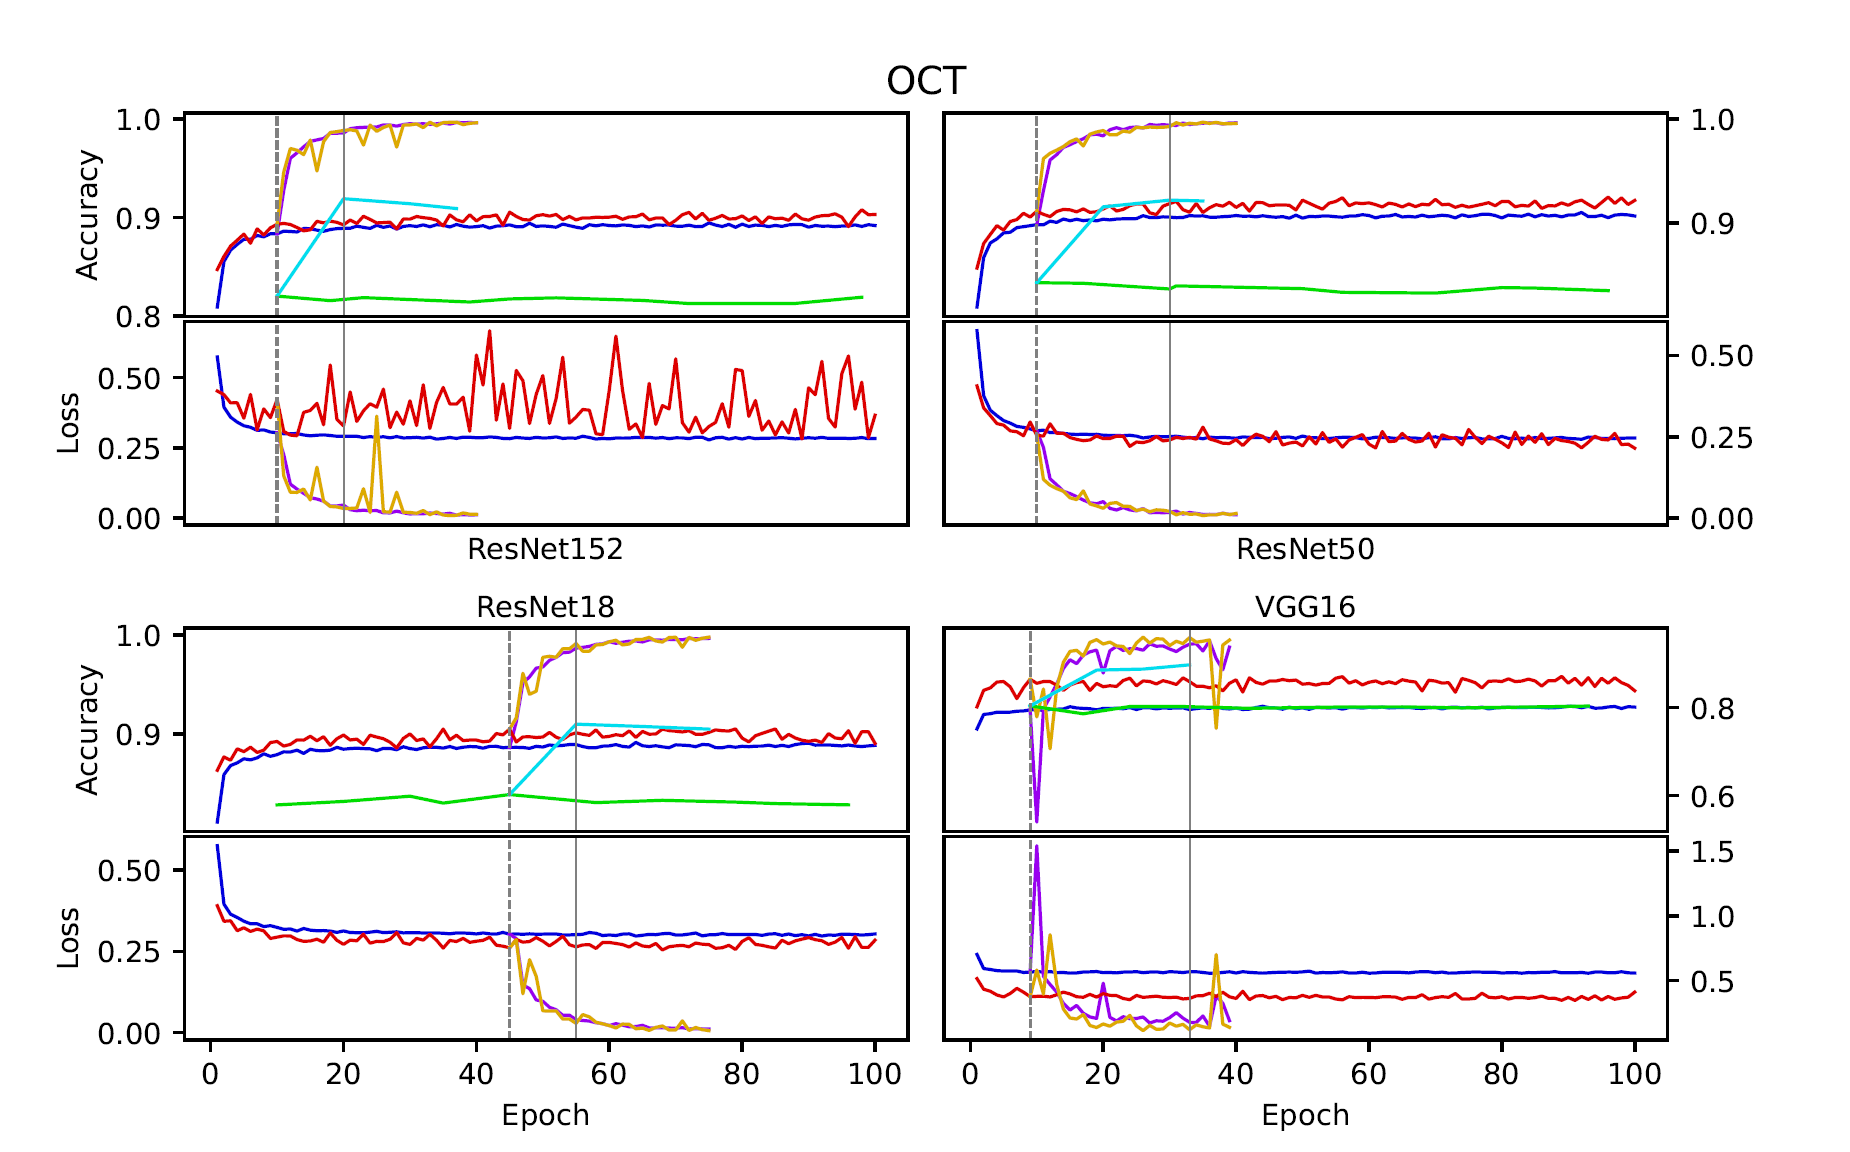
\includegraphics[width=\linewidth]{Figs/abnormity_OCT_loss_and_acc.png}
			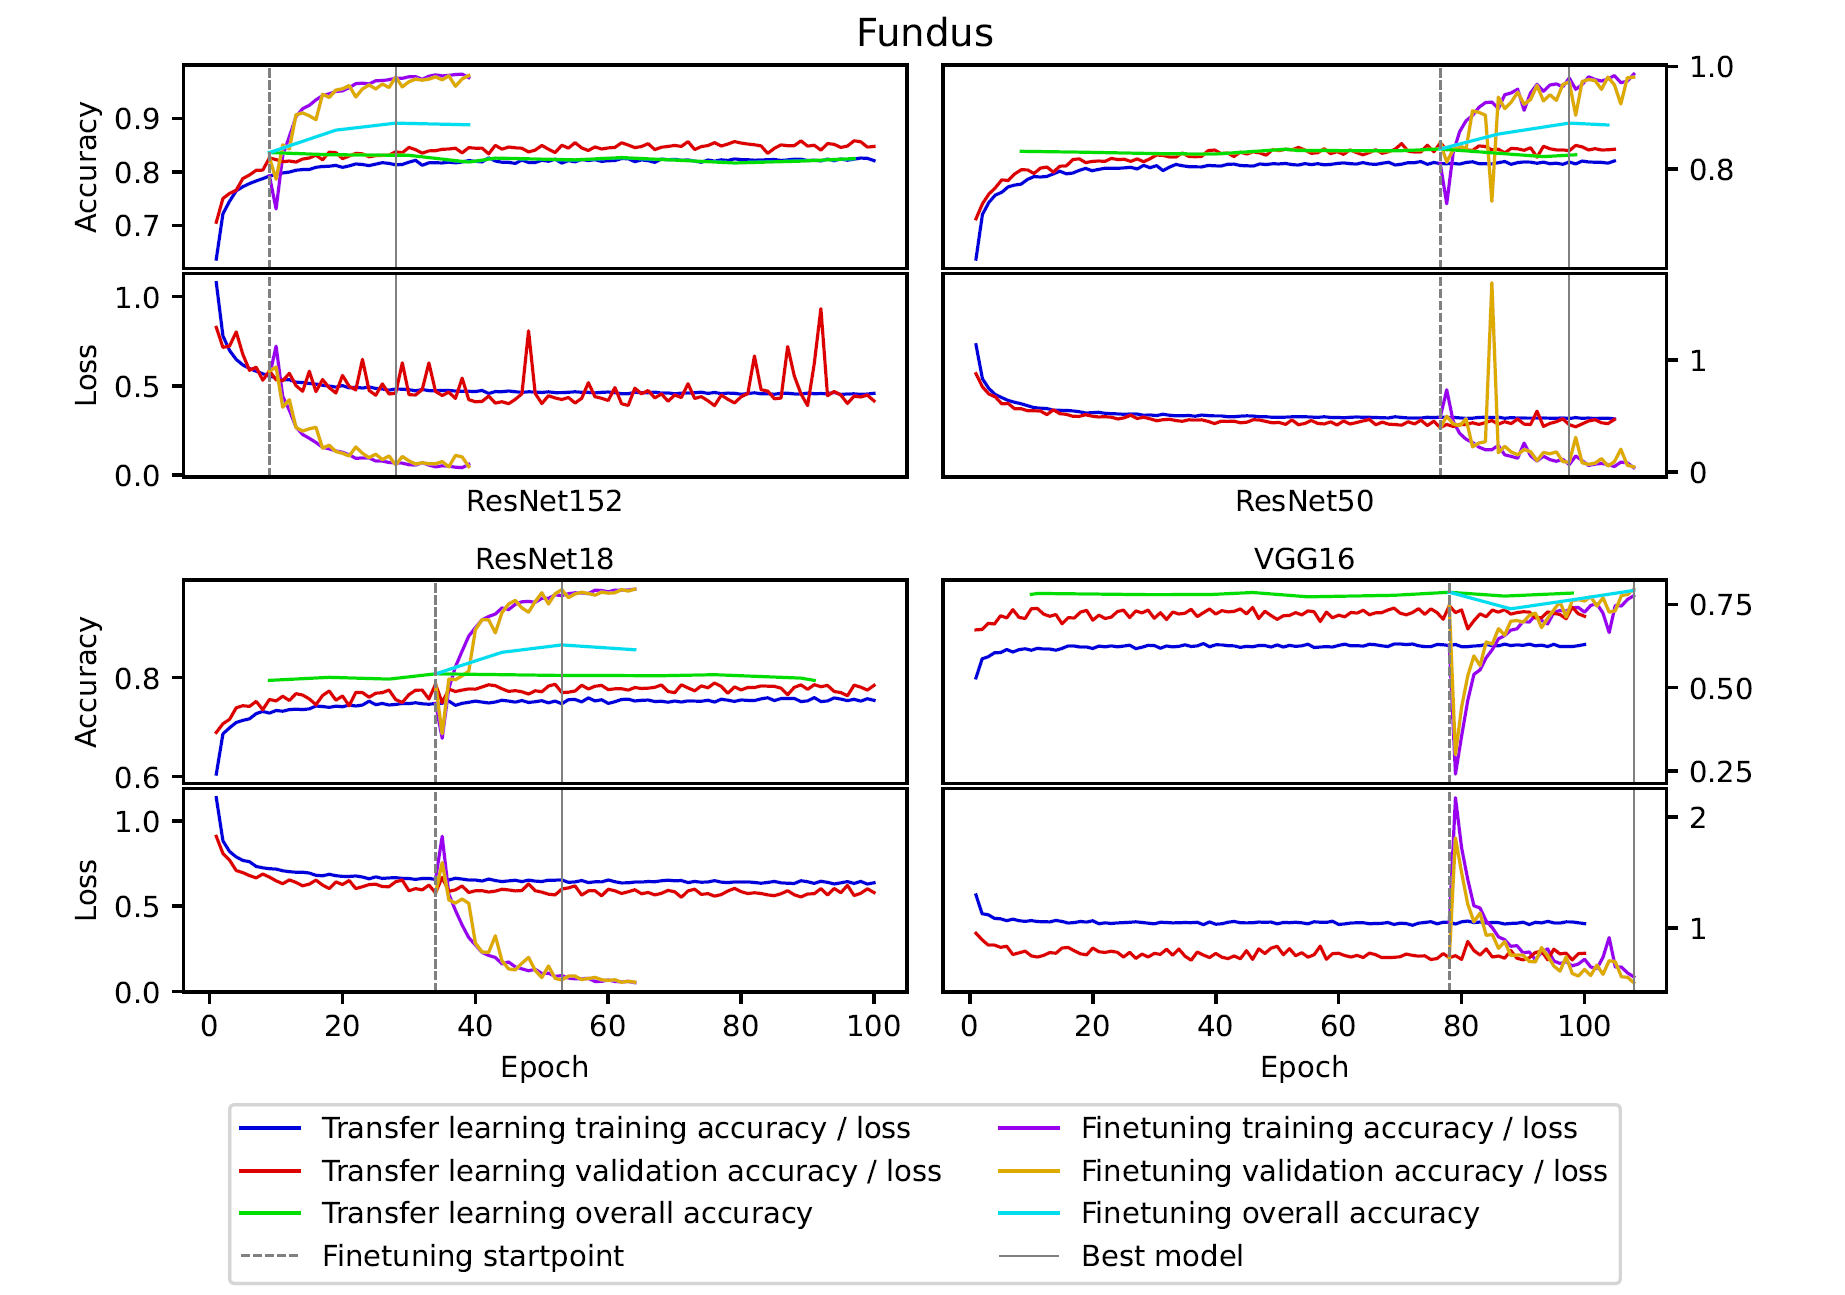
\includegraphics[width=\linewidth]{Figs/abnormity_Fundus_loss_and_acc.png}
			\caption{异常模型训练}
			\label{fig:A_train}
		\end{figure}
		
		\pagebreak
		
		{
		\fontsize{9}{12}\selectfont
		{
			\begin{table}
				\centering
				\caption{使用不同CNN的总体准确率}
				\label{tb:A_accuracies}
				\begin{tabular}{ccccc}
					\toprule
					模型&ResNet152&ResNet50&ResNet18&VGG16\\
					\midrule
					OCT模型   &91.906\%&\textbf{92.183\%}&91.011\%&89.744\% \\
					眼底模型&\textbf{89.111\%}&88.926\%&86.605\%&79.185\% \\
					\bottomrule
				\end{tabular}
			\end{table}
		}
		}	
		
		\begin{table}[htbp]
			\centering
			\fontsize{9}{12}\selectfont{
			\caption{OCT模型的测试结果}
			\label{tb:OCT_test}
			\pgfplotstabletypeset[
			multicolumn names,
			col sep=comma,
			columns = {Abnormity, Precision, Sensitivity, Specificity, FOne, AUC},
			columns/Abnormity/.style={string type, column name=异常},
			columns/Precision/.style={string type, column name=精确率},
			columns/Sensitivity/.style={string type, column name=敏感性},
			columns/Specificity/.style={string type, column name=特异性},
			columns/FOne/.style={string type, column name={F1分数}},
			columns/AUC/.style={string type, column name=AUC},
			every head row/.style={before row=\toprule, after row=\midrule},
			every last row/.style={ after row=\bottomrule}
			]{Tables/abnormity_o_test.csv}}
		\end{table}
		\begin{table}[H]
			\centering
			\fontsize{9}{12}\selectfont{
			\caption{眼底模型的测试结果}
			\label{tb:Fundus_test}
			\pgfplotstabletypeset[
			multicolumn names,
			col sep=comma,
			columns = {Abnormity, Precision, Sensitivity, Specificity, FOne, AUC},
			columns/Abnormity/.style={string type, column name=异常},
			columns/Precision/.style={string type, column name=精确率},
			columns/Sensitivity/.style={string type, column name=敏感性},
			columns/Specificity/.style={string type, column name=特异性},
			columns/FOne/.style={string type, column name={F1分数}},
			columns/AUC/.style={string type, column name=AUC},
			every head row/.style={before row=\toprule, after row=\midrule},
			every last row/.style={after row=\bottomrule}
			]{Tables/abnormity_f_test.csv}}
		\end{table}
		
		\pagebreak
	
		\begin{figure}[htbp]
			\vspace{3.5cm}
			\centering
			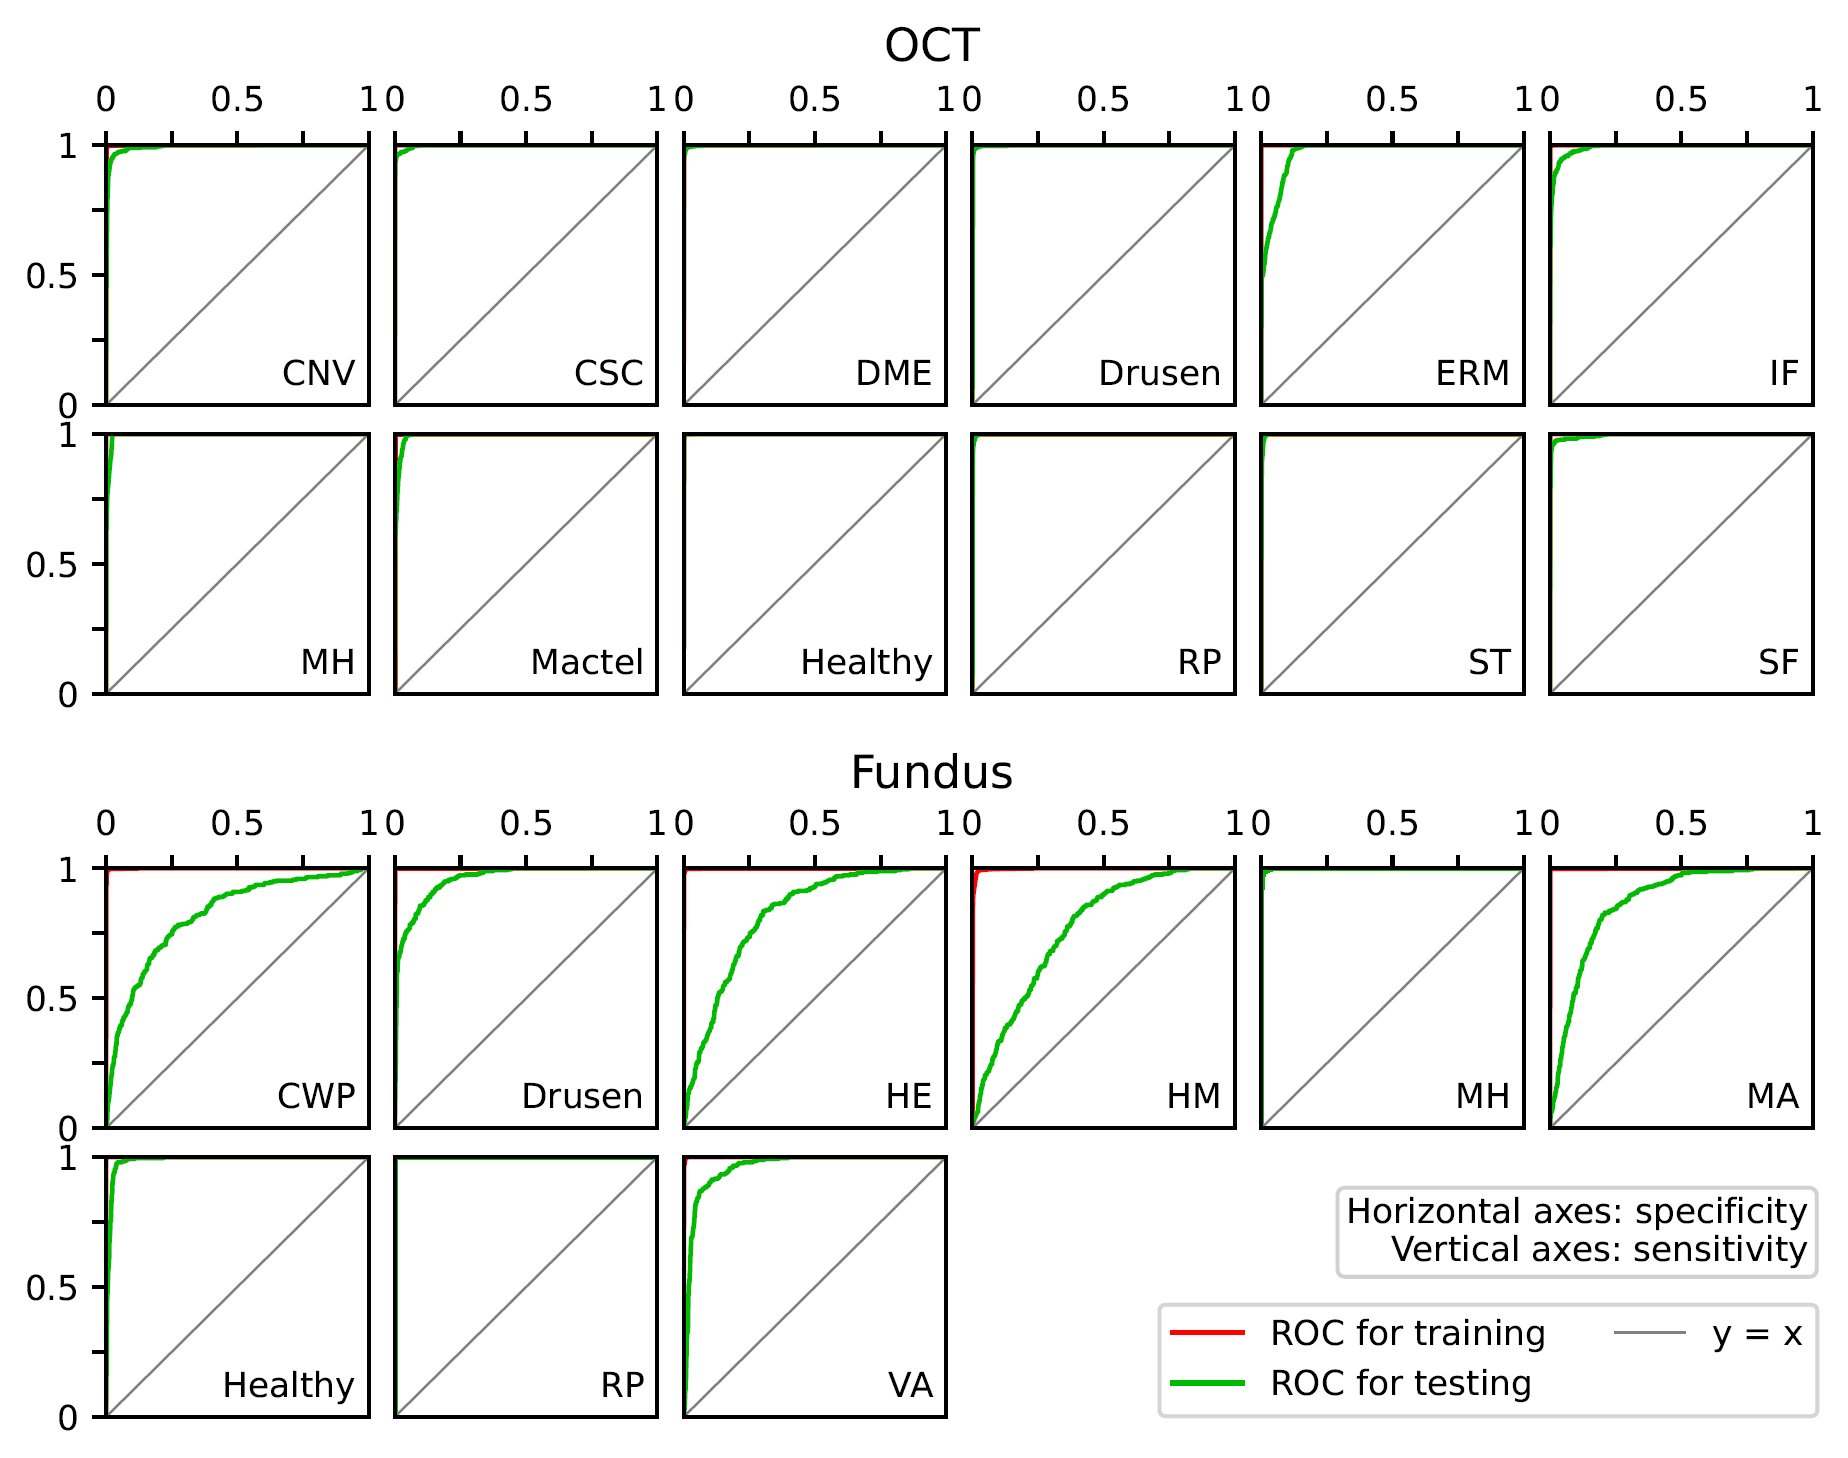
\includegraphics[width=\linewidth]{Figs/abnormity_ROC.png}
			\caption{异常模型的ROC曲线}
			\vspace{0.3cm}
			\label{fig:A_ROC}
		\end{figure}
		
		\begin{figure}[htbp]
			\centering
			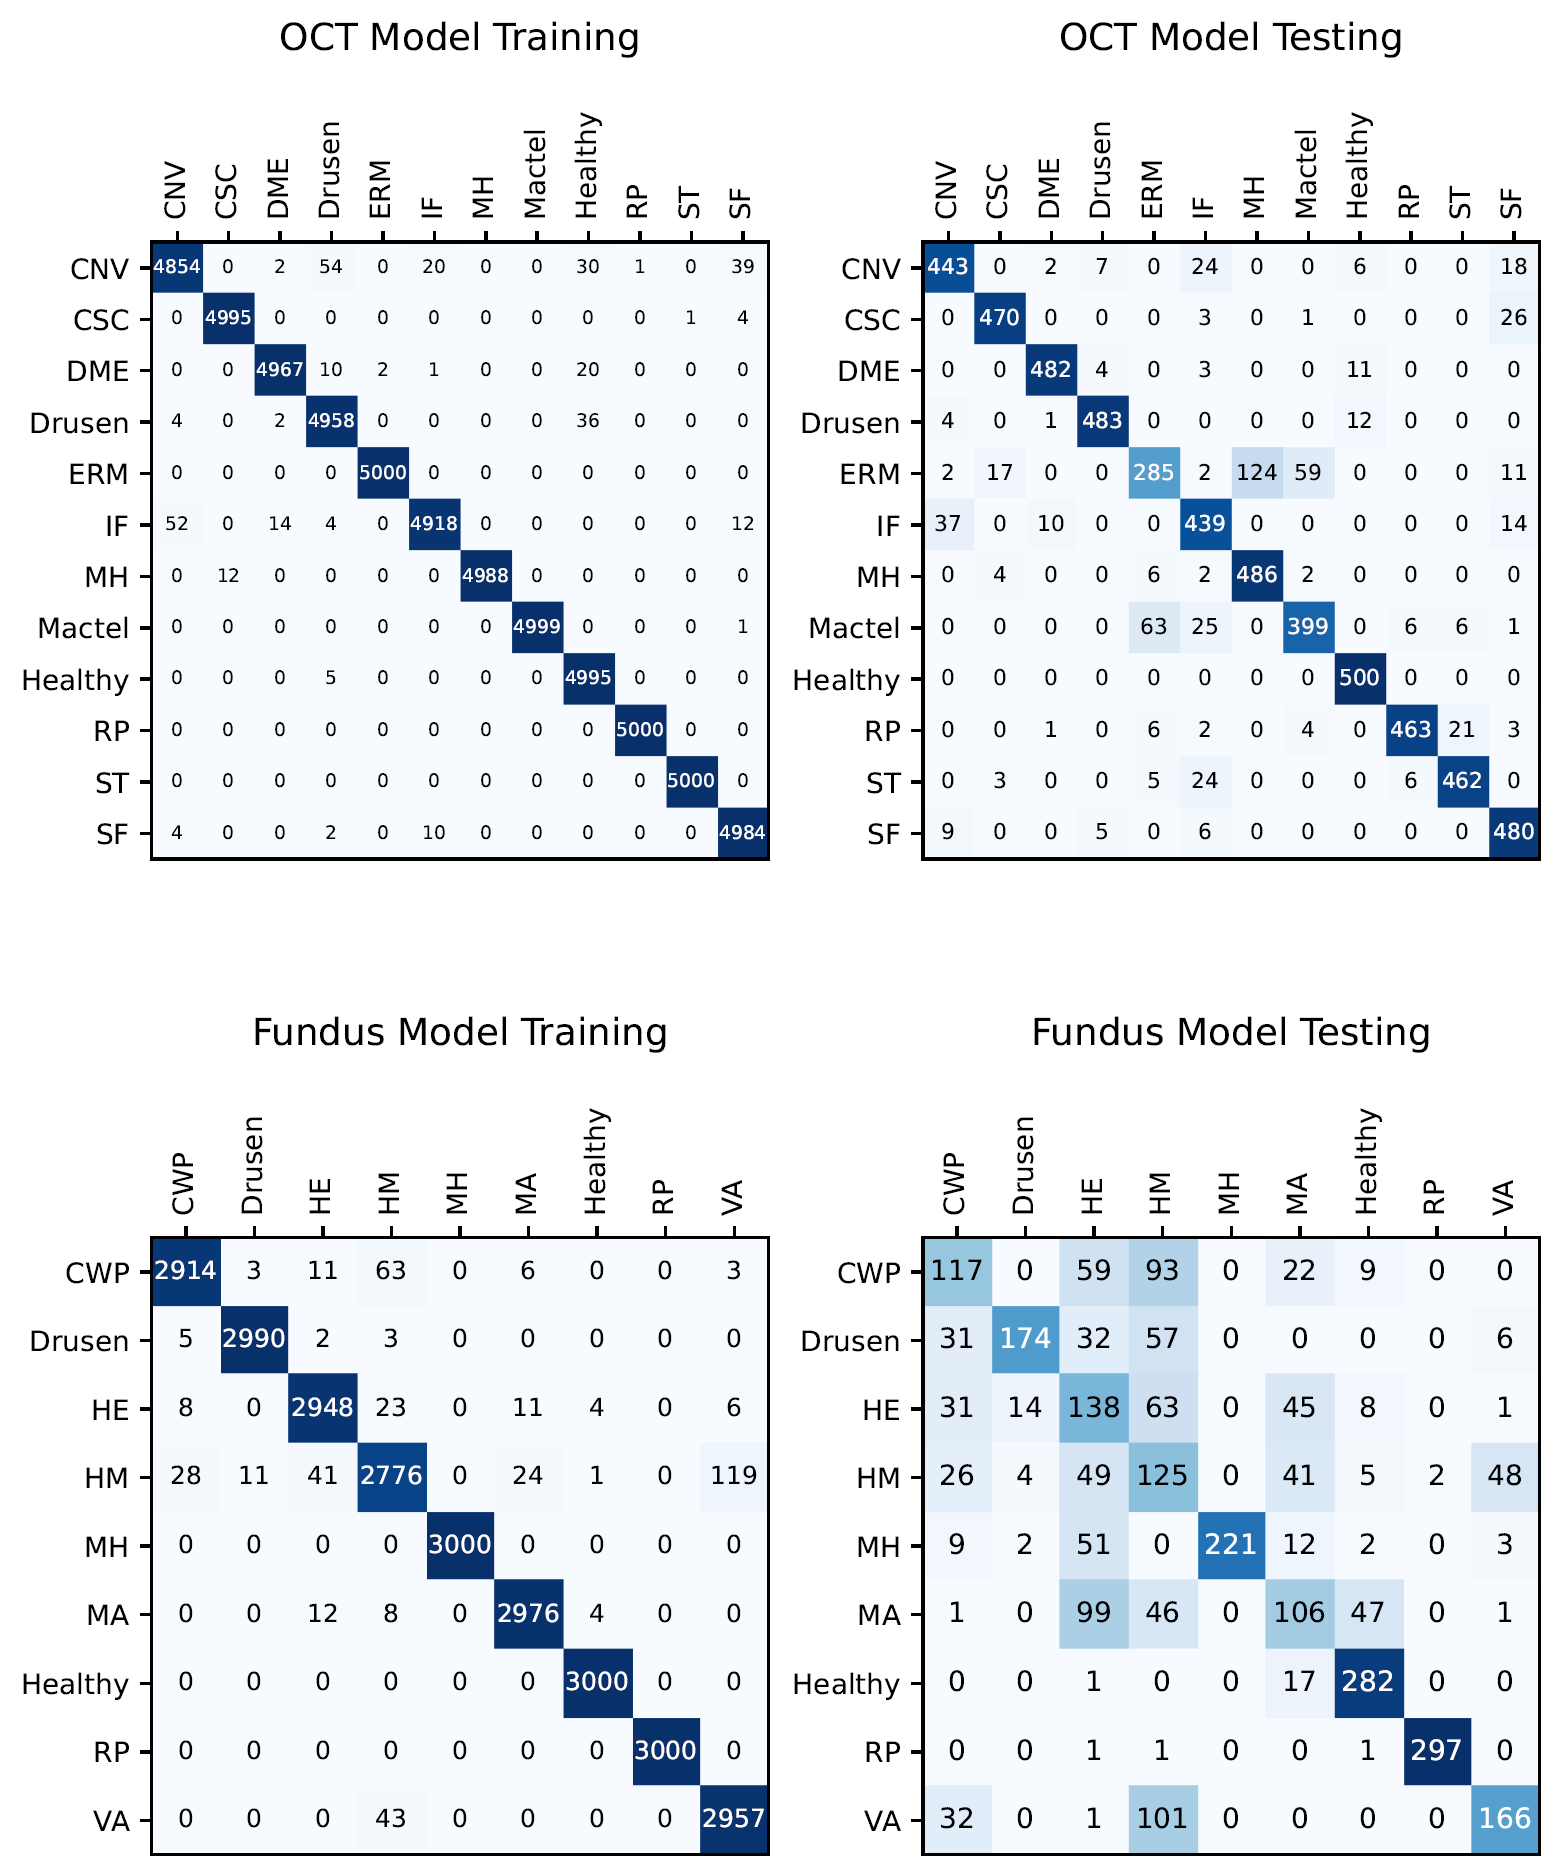
\includegraphics[width=\linewidth]{Figs/abnormity_confusion_matrix.png}
			\caption{异常模型的混淆矩阵}
			\vspace{0.3cm}
			\label{fig:A_conf_mat}
		\end{figure}
		
		\begin{figure}[htbp]
			\centering
			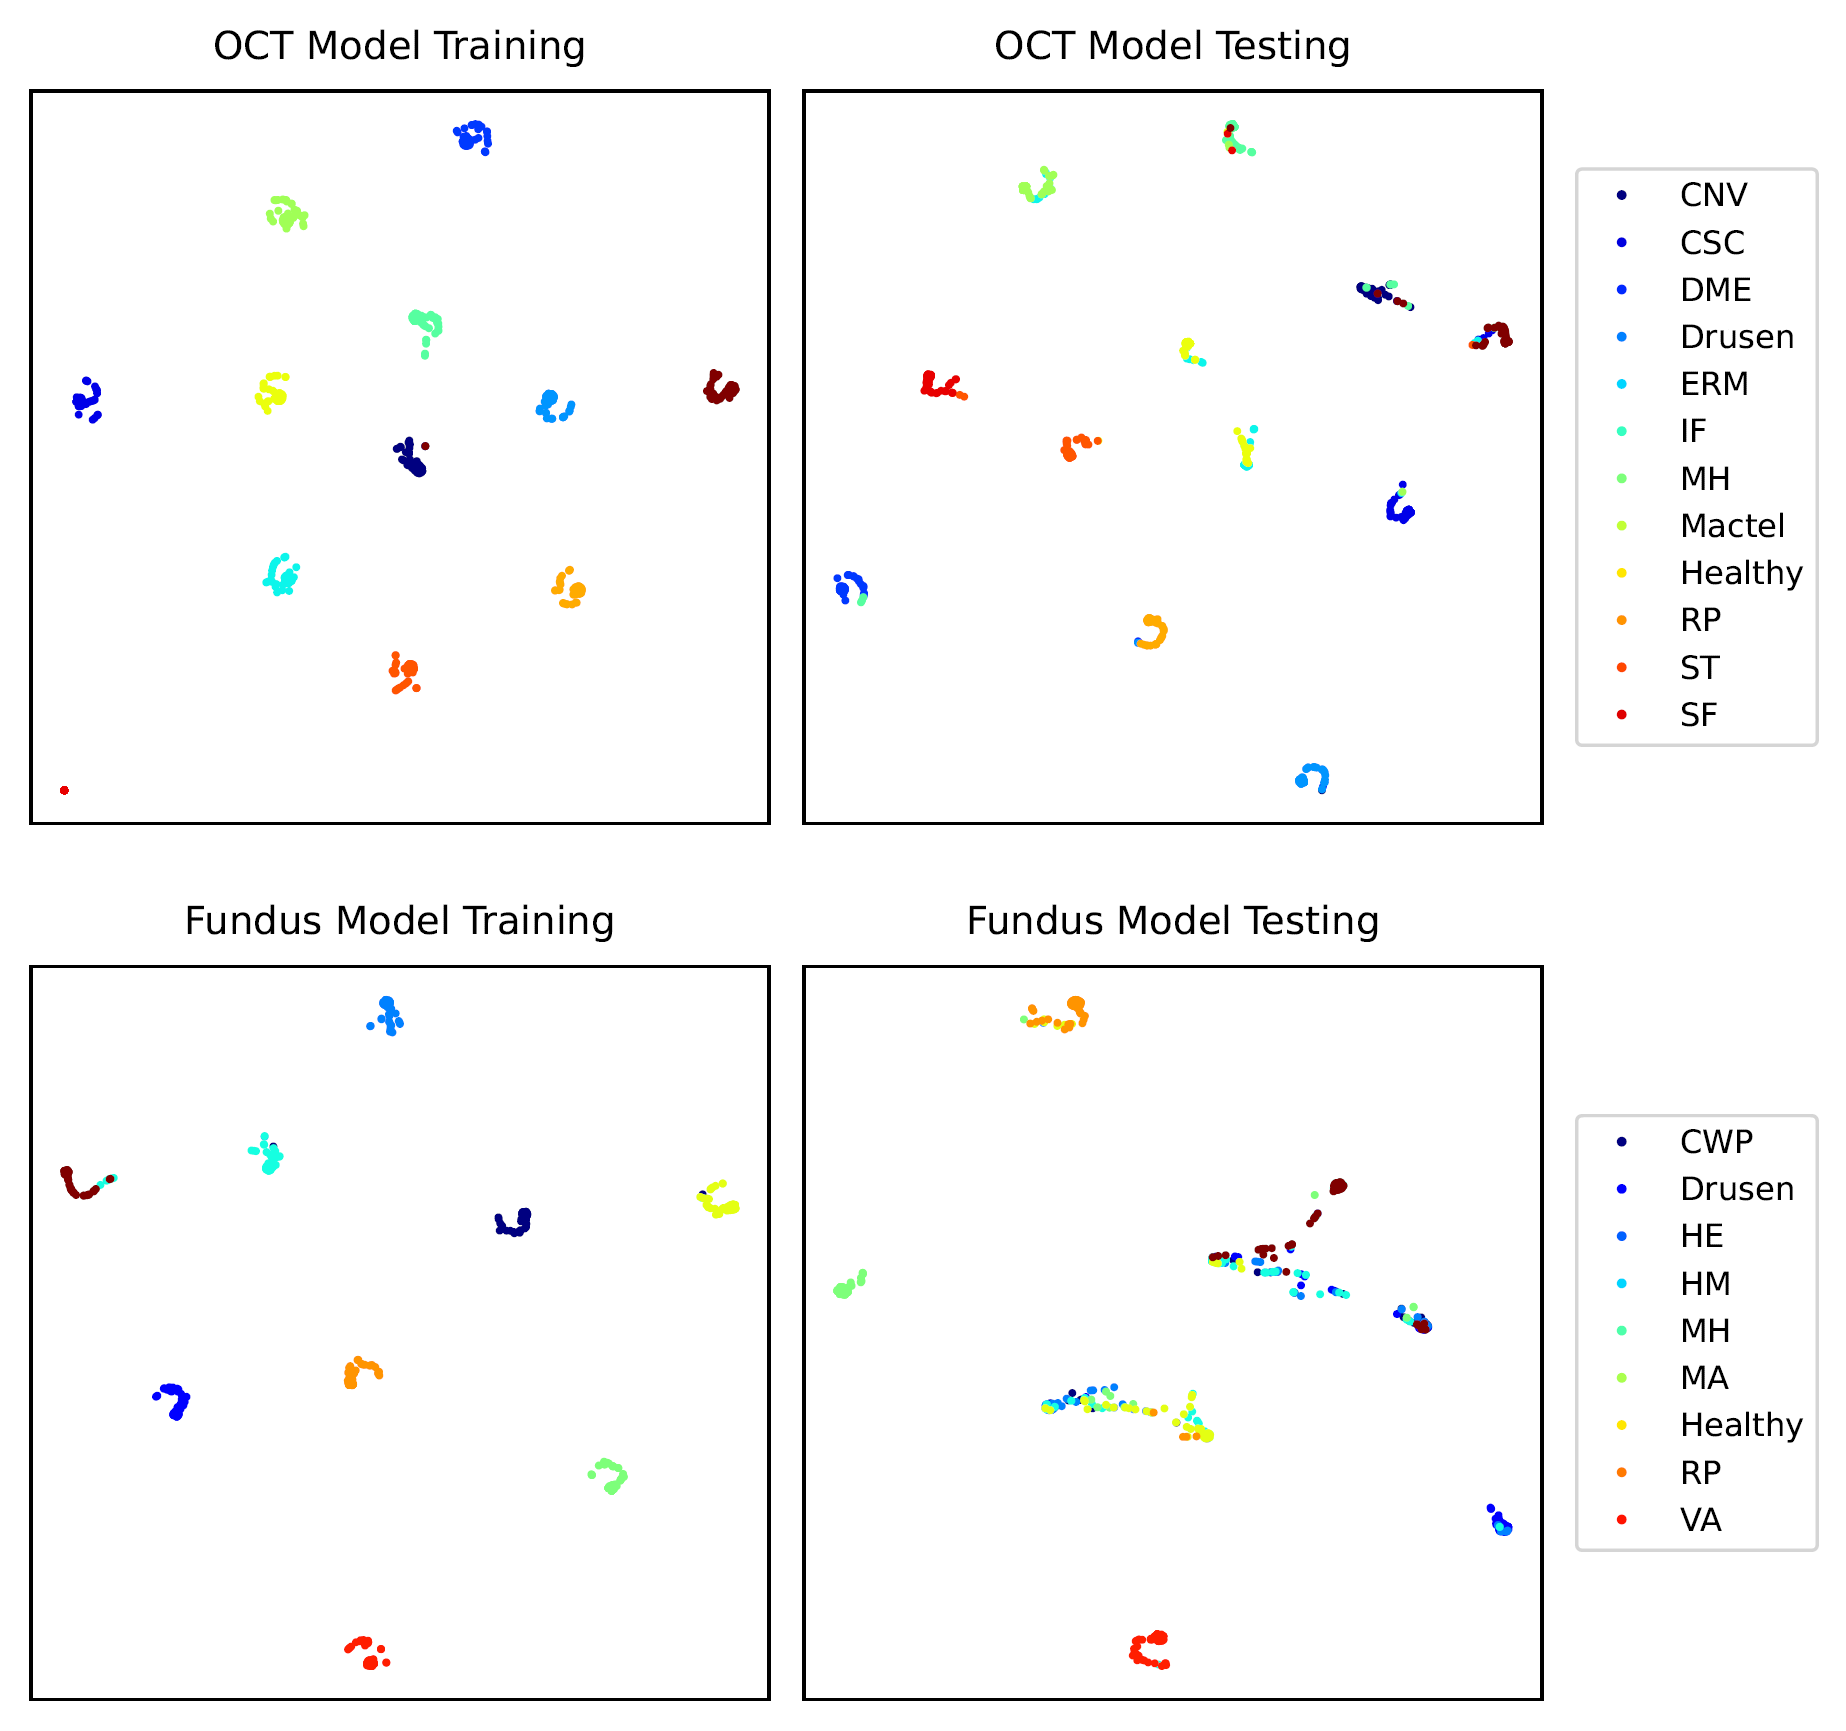
\includegraphics[width=\linewidth]{Figs/abnormity_tSNE.png}
			\caption{异常模型的t-SNE图}
			\vspace{0.3cm}
			\label{fig:A_tSNE}
		\end{figure}
		
		\begin{figure}[htbp]
			\centering
			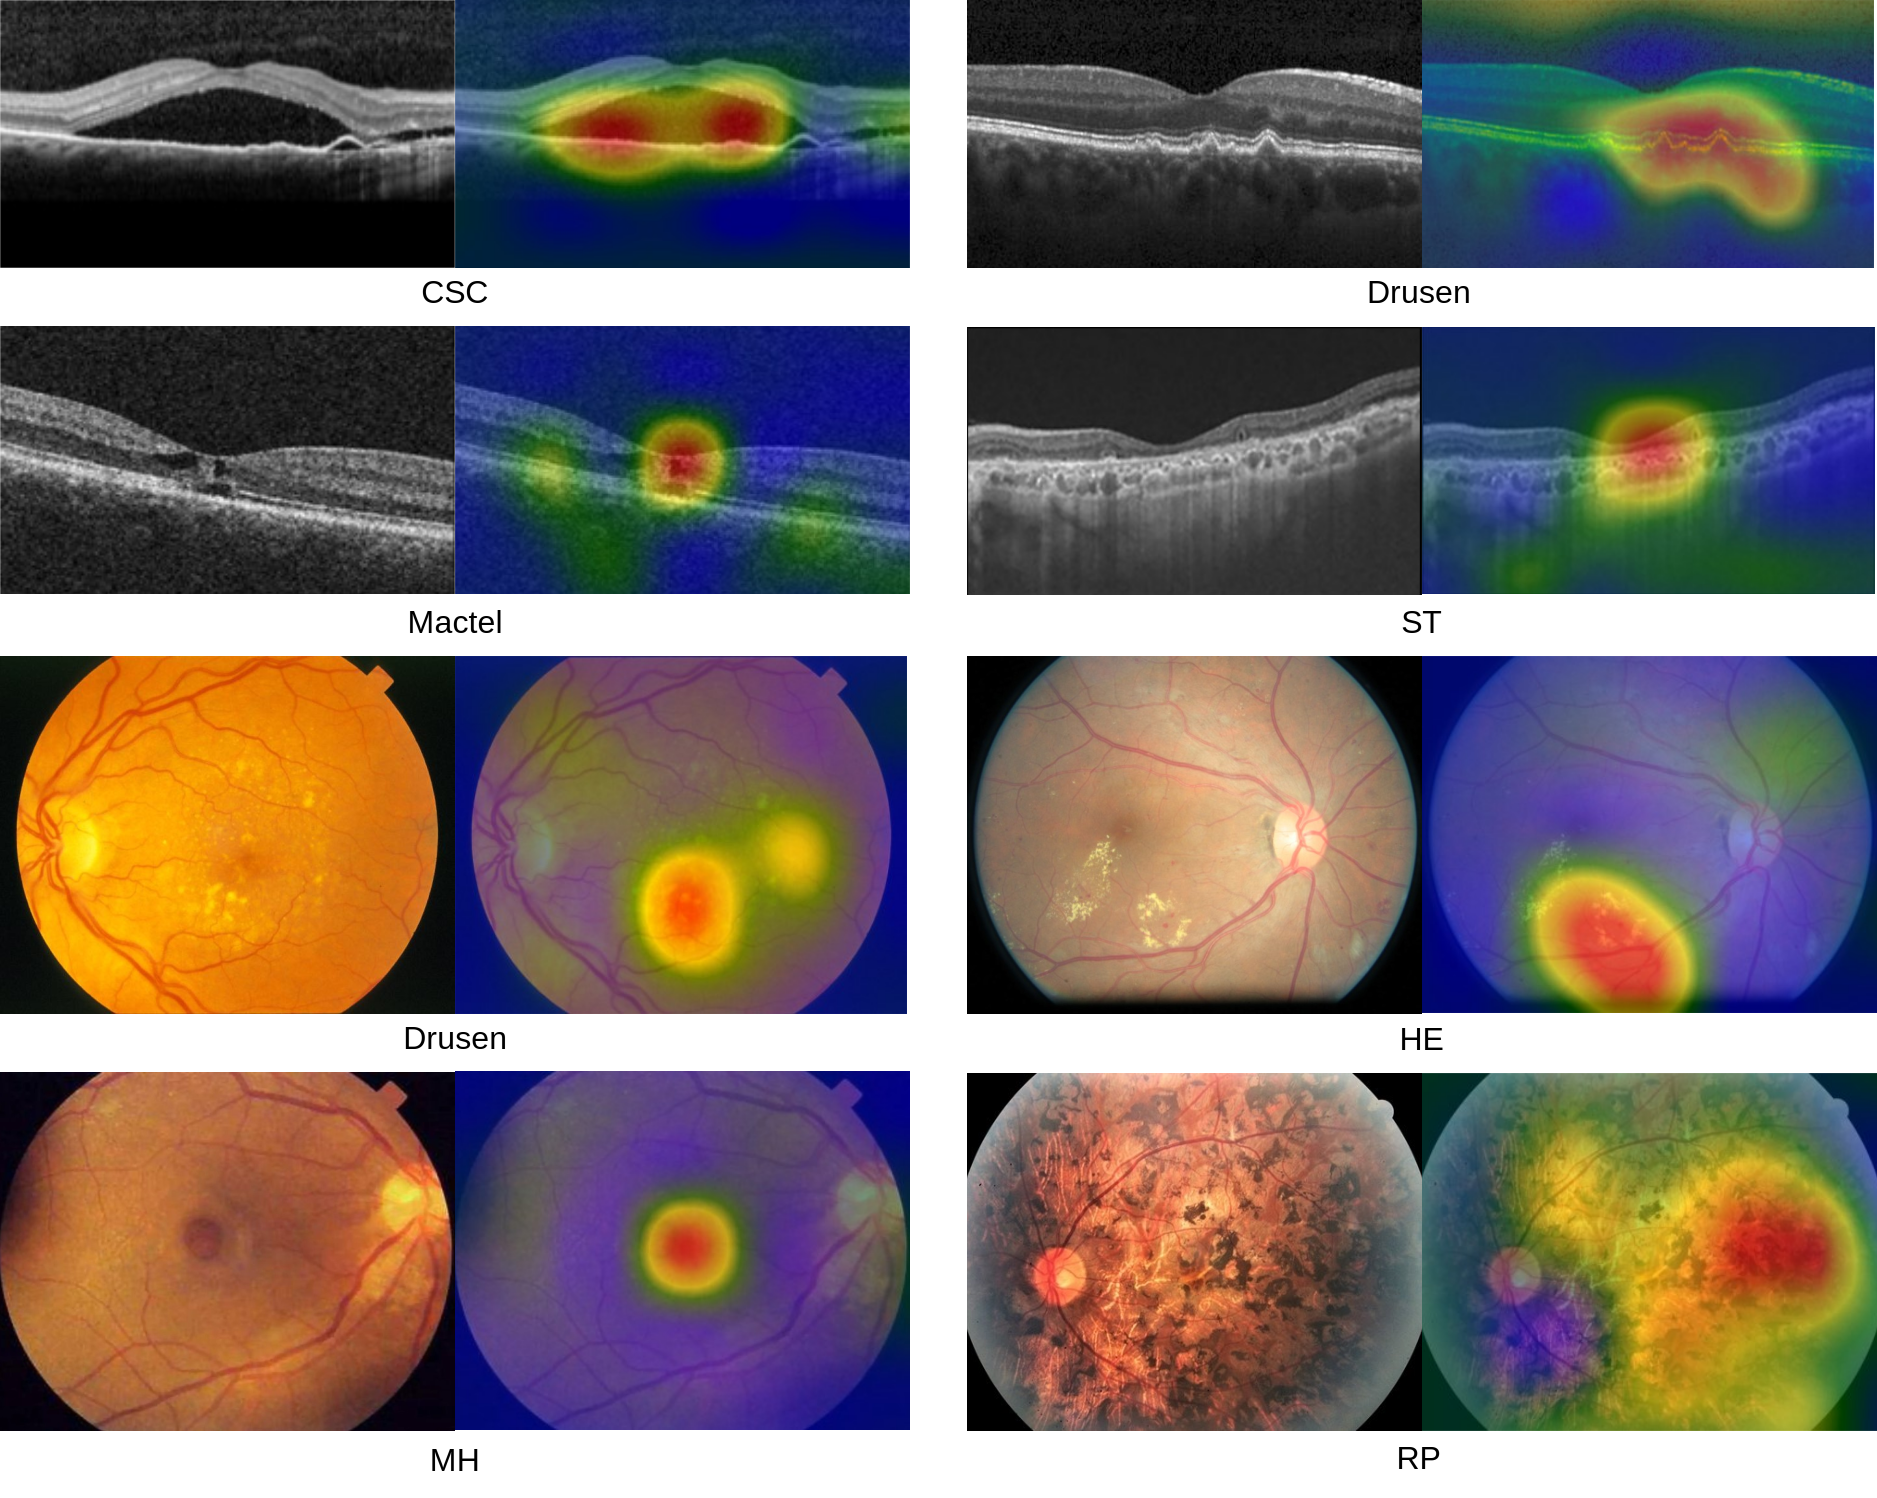
\includegraphics[width=\linewidth]{Figs/abnormity_gradCAM.png}
			\caption{Grad-CAM高亮显示异常}
			\vspace{0.3cm}
			\label{fig:gradCAM}
		\end{figure}
		
		\begin{figure}[htbp]
			\centering
			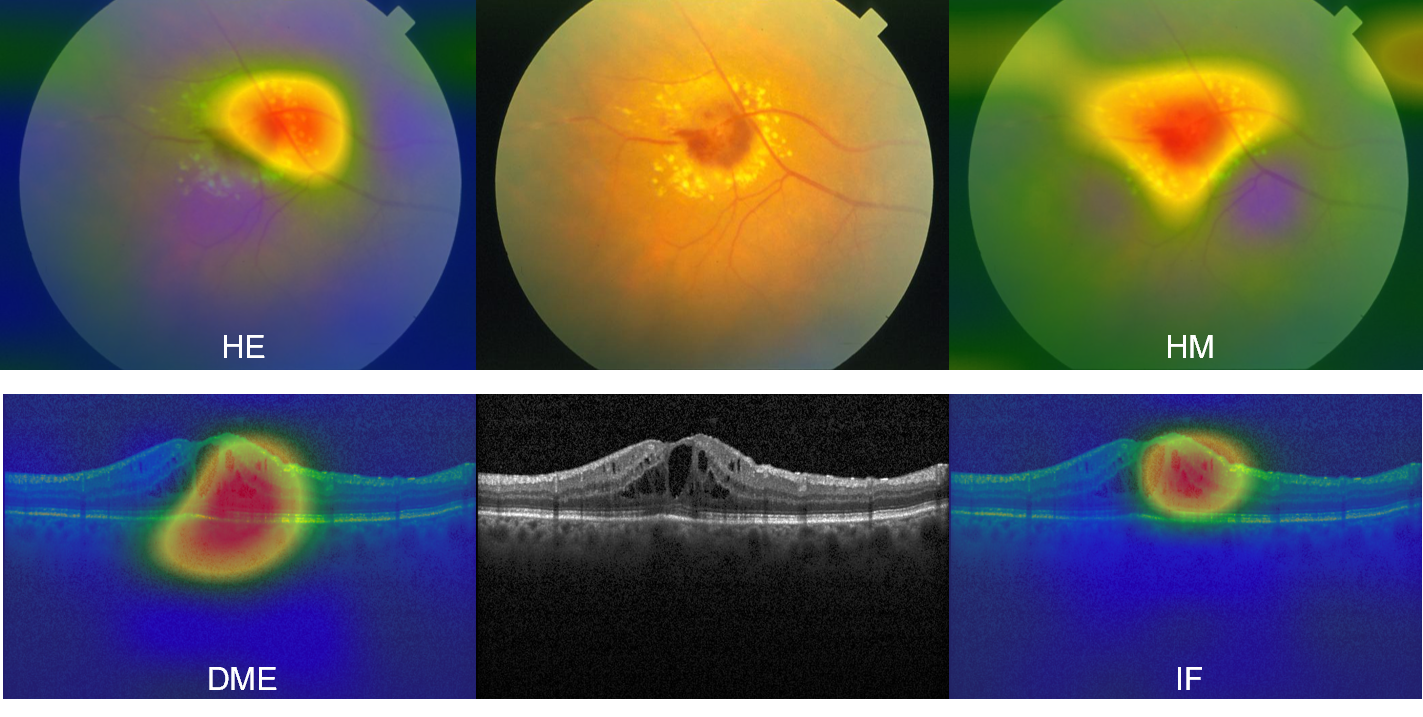
\includegraphics[width=0.8\linewidth]{Figs/abnormity_gradCAM_multiple_abnormities.png}
			\caption{Grad-CAM高亮显示多处异常}
			\vspace{0.3cm}
			\label{fig:gradCAM_multi_abnormity}
		\end{figure}
	
		\vspace{1.5cm}
	
	
		
	\pagebreak	
	
	\begin{multicols}{2}
	\section{诊断模型}
	
	\subsection{数据准备}
	
	阶段 D1 的目的是确定每种疾病的严重程度,每种疾病对应一个子模型。我们根据异常-疾病推导标准(见图~\ref{fig:criteria})为每个子模型准备数据。如第~\ref{sec:overview}~节所述,我们确定一种疾病的目标异常,并根据目标异常的数量定义严重程度。如果某种疾病有 5 个目标异常,则考虑到健康状态,共有 6 个严重程度级别,即 0 至 5。我们使用一组图像作为子模型的输入,每组图像的严重程度标签等于该组中出现的目标异常数量。我们随机选择 OCT 和眼底图像集,为每组确定严重程度。最终,我们为每个严重程度获得 10000 组训练输入和 10000 组测试输入。
	
	阶段 D2 的目的是输出疾病概率向量。对于每种疾病,我们使用异常-疾病推导标准找到目标异常,随机选择每个目标异常的一组图像,将这些图像集标记为该疾病。我们为每种疾病获取了 10000 组训练图像集和 10000 组测试图像集。
	
	\subsection{训练}
	
	诊断模型与异常模型使用相同的硬件进行训练。阶段 D1 子模型训练 10 个 epoch,阶段 D2 模型训练 30 个 epoch,其余超参数与异常模型相同,详情参见第~\ref{sec:a_training}~节。
	
	阶段 D1 的子模型和阶段 D2 的模型在训练和验证过程中迅速达到较高的准确率,因为训练数据充足,且模型结构相对简单。
	
	
	\subsection{结果}
	
	图~\ref{fig:D1_acc_bar} 显示了阶段 D1 子模型的准确率,图~\ref{fig:D1_conf_mat} 显示了阶段 D1 的混淆矩阵。表~\ref{tb:diagnosis_test} 显示了阶段 D2 的预测值,图~\ref{fig:D2_ROC} 显示了 ROC 曲线,图~\ref{fig:D2_conf_mat} 显示了混淆矩阵,图~\ref{fig:D2_tSNE} 显示了 t-SNE 图。
	
	阶段 D1 的子模型在预测结果上常常比标签偏差一个级别,这降低了阶段 D1 子模型的准确率。然而,阶段 D2 部分解决了此问题,因为阶段 D2 模型的准确率高于阶段 D1 子模型的平均准确率。
	
	阶段 D2 在疾病分类方面表现相当出色。考虑到某些疾病可能相似,我们使用了类似共显异常的方法,使阶段 D2 能够输出最多 3 个共显疾病。正如图~\ref{fig:D1_acc_bar} 所示,若使用共显疾病方法,阶段 D2 的准确率进一步提高。
	\end{multicols}
	
	\begin{figure}[htbp]
		\centering
		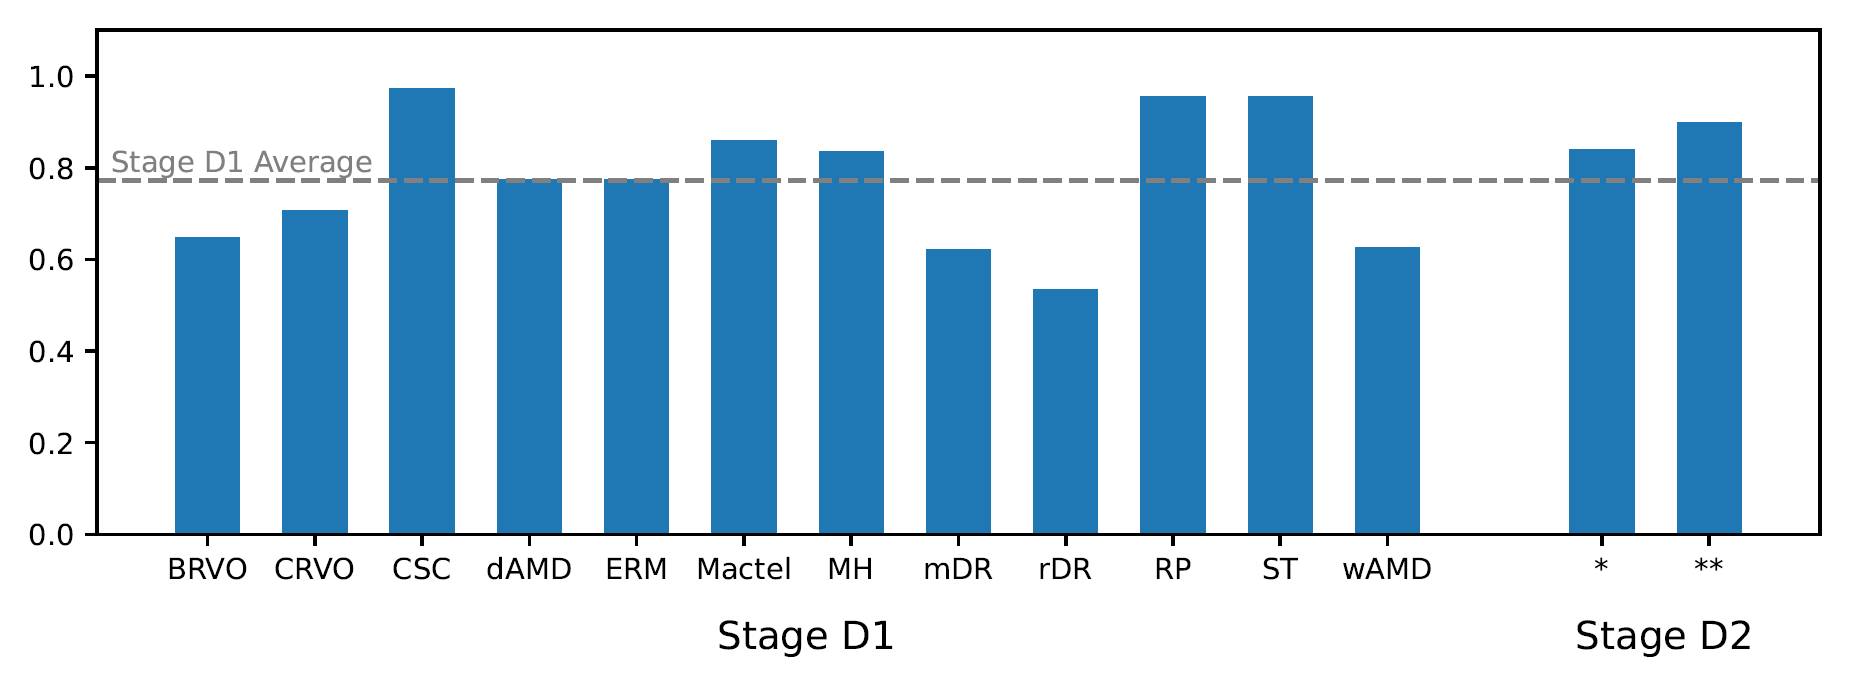
\includegraphics[width=\linewidth]{Figs/diagnosis1_acc_barchart.png}
		\caption{诊断模型的准确率(*:只取概率最高的疾病的准确率;**:考虑共显疾病的准确率)}
		\vspace{0.3cm}
		\label{fig:D1_acc_bar}
	\end{figure}
	
	\begin{figure}[htbp]
		\centering
		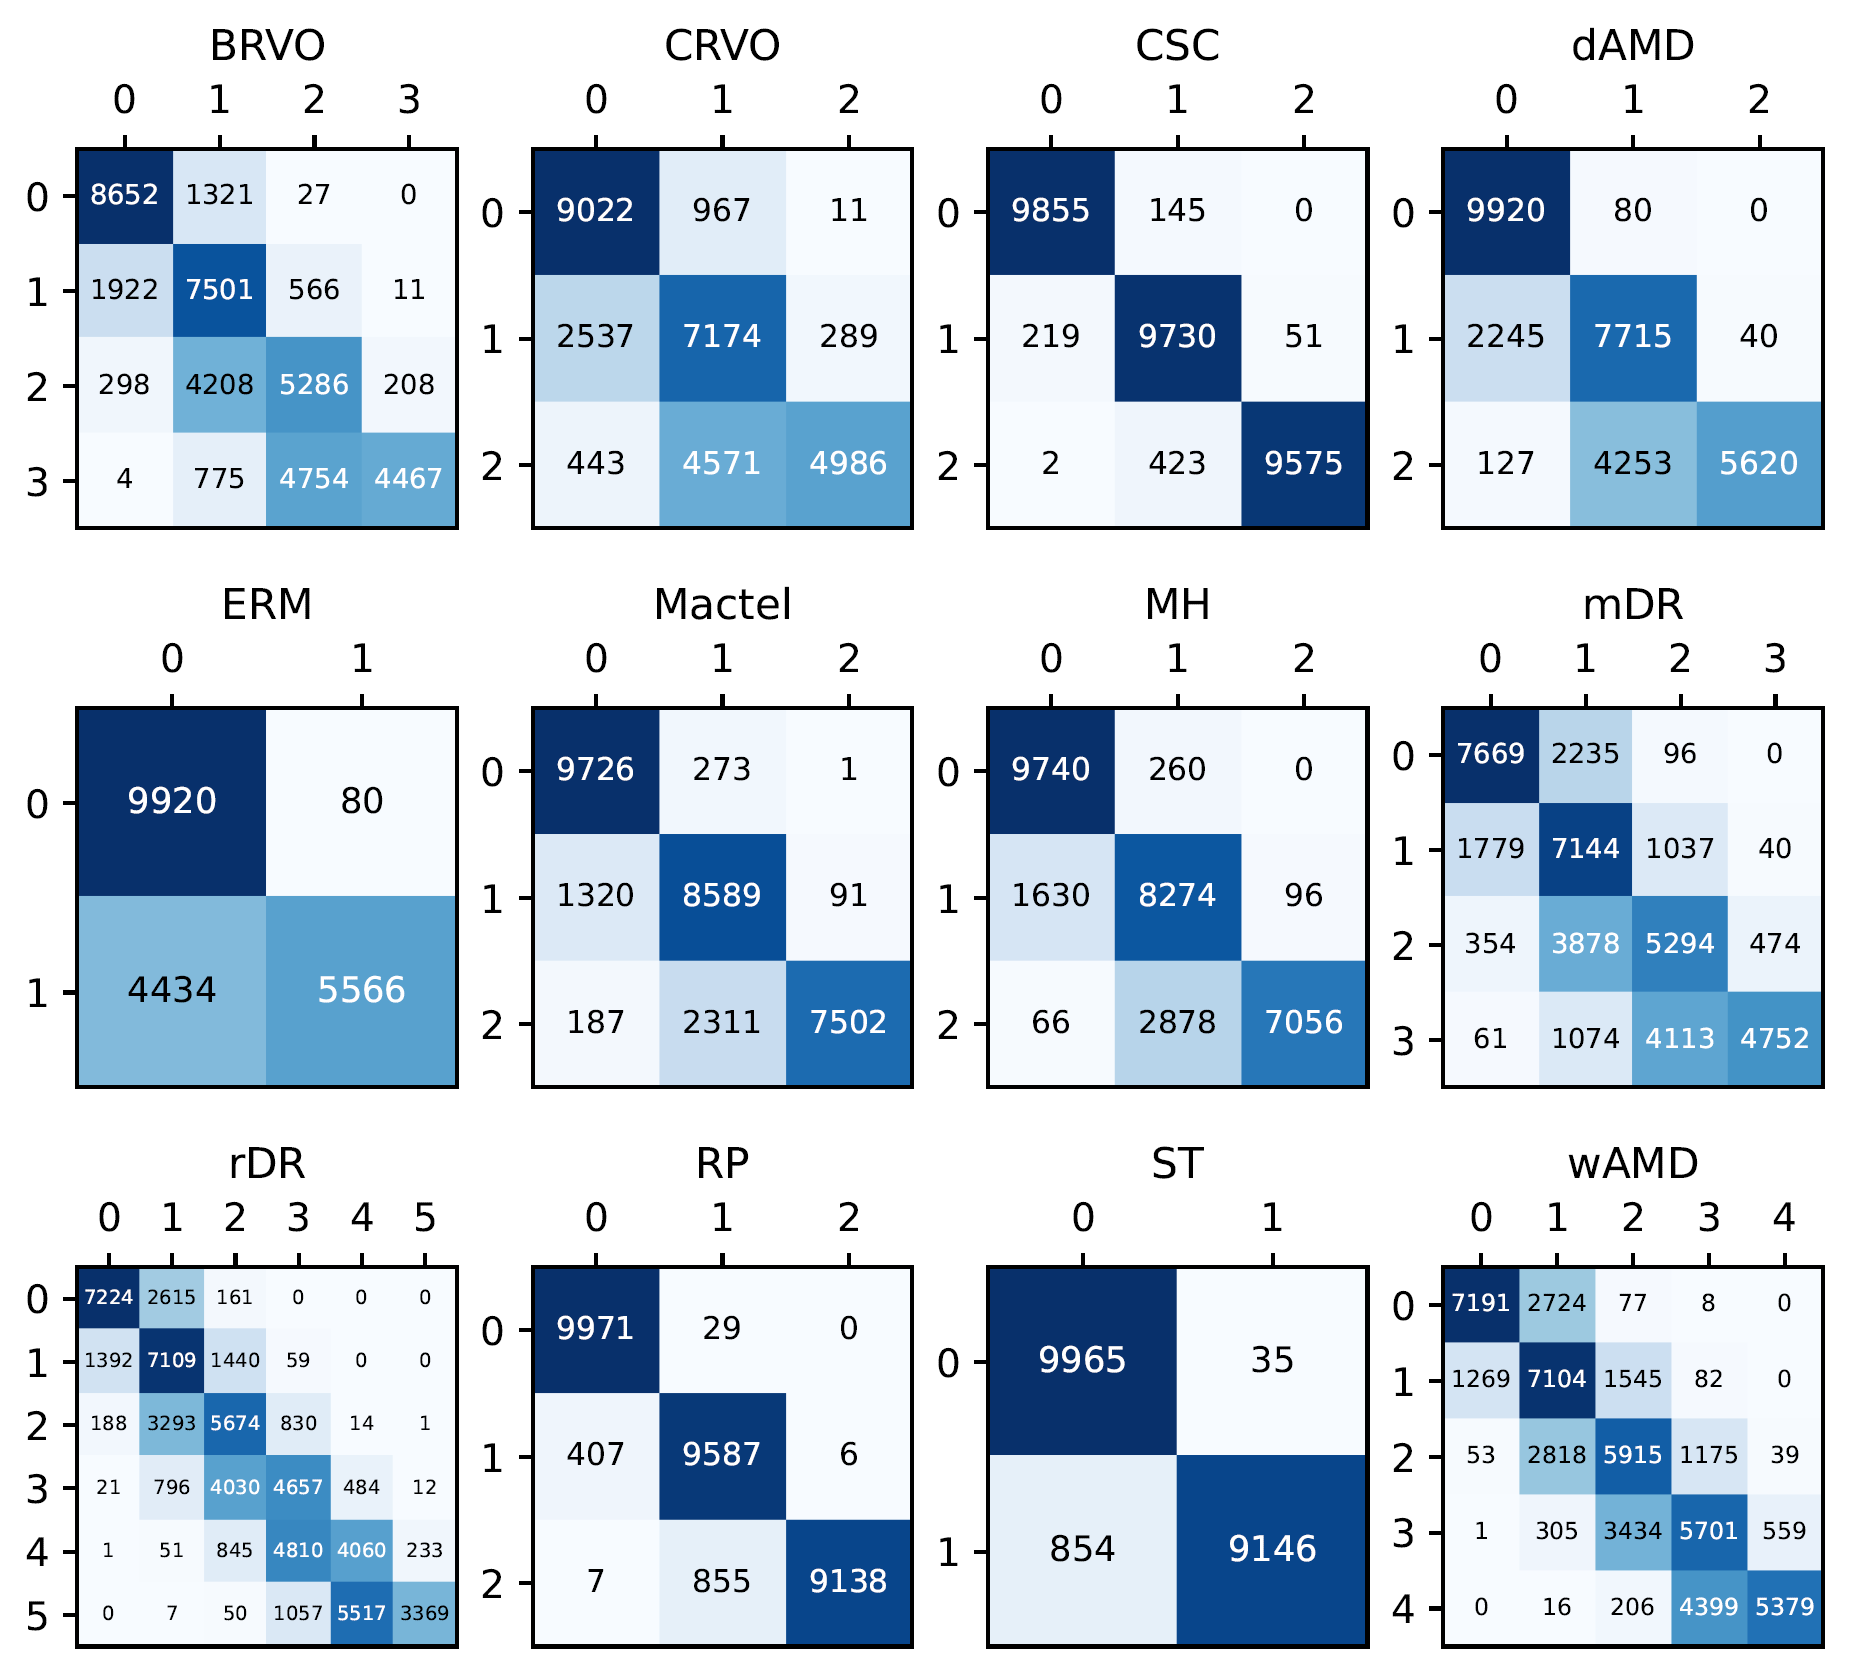
\includegraphics[width=\linewidth]{Figs/diagnosis1_confusion_matrix.png}
		\caption{阶段D1的混淆矩阵}
		\vspace{0.3cm}
		\label{fig:D1_conf_mat}
	\end{figure}
	
	
	\begin{figure}[htbp]
		\centering
		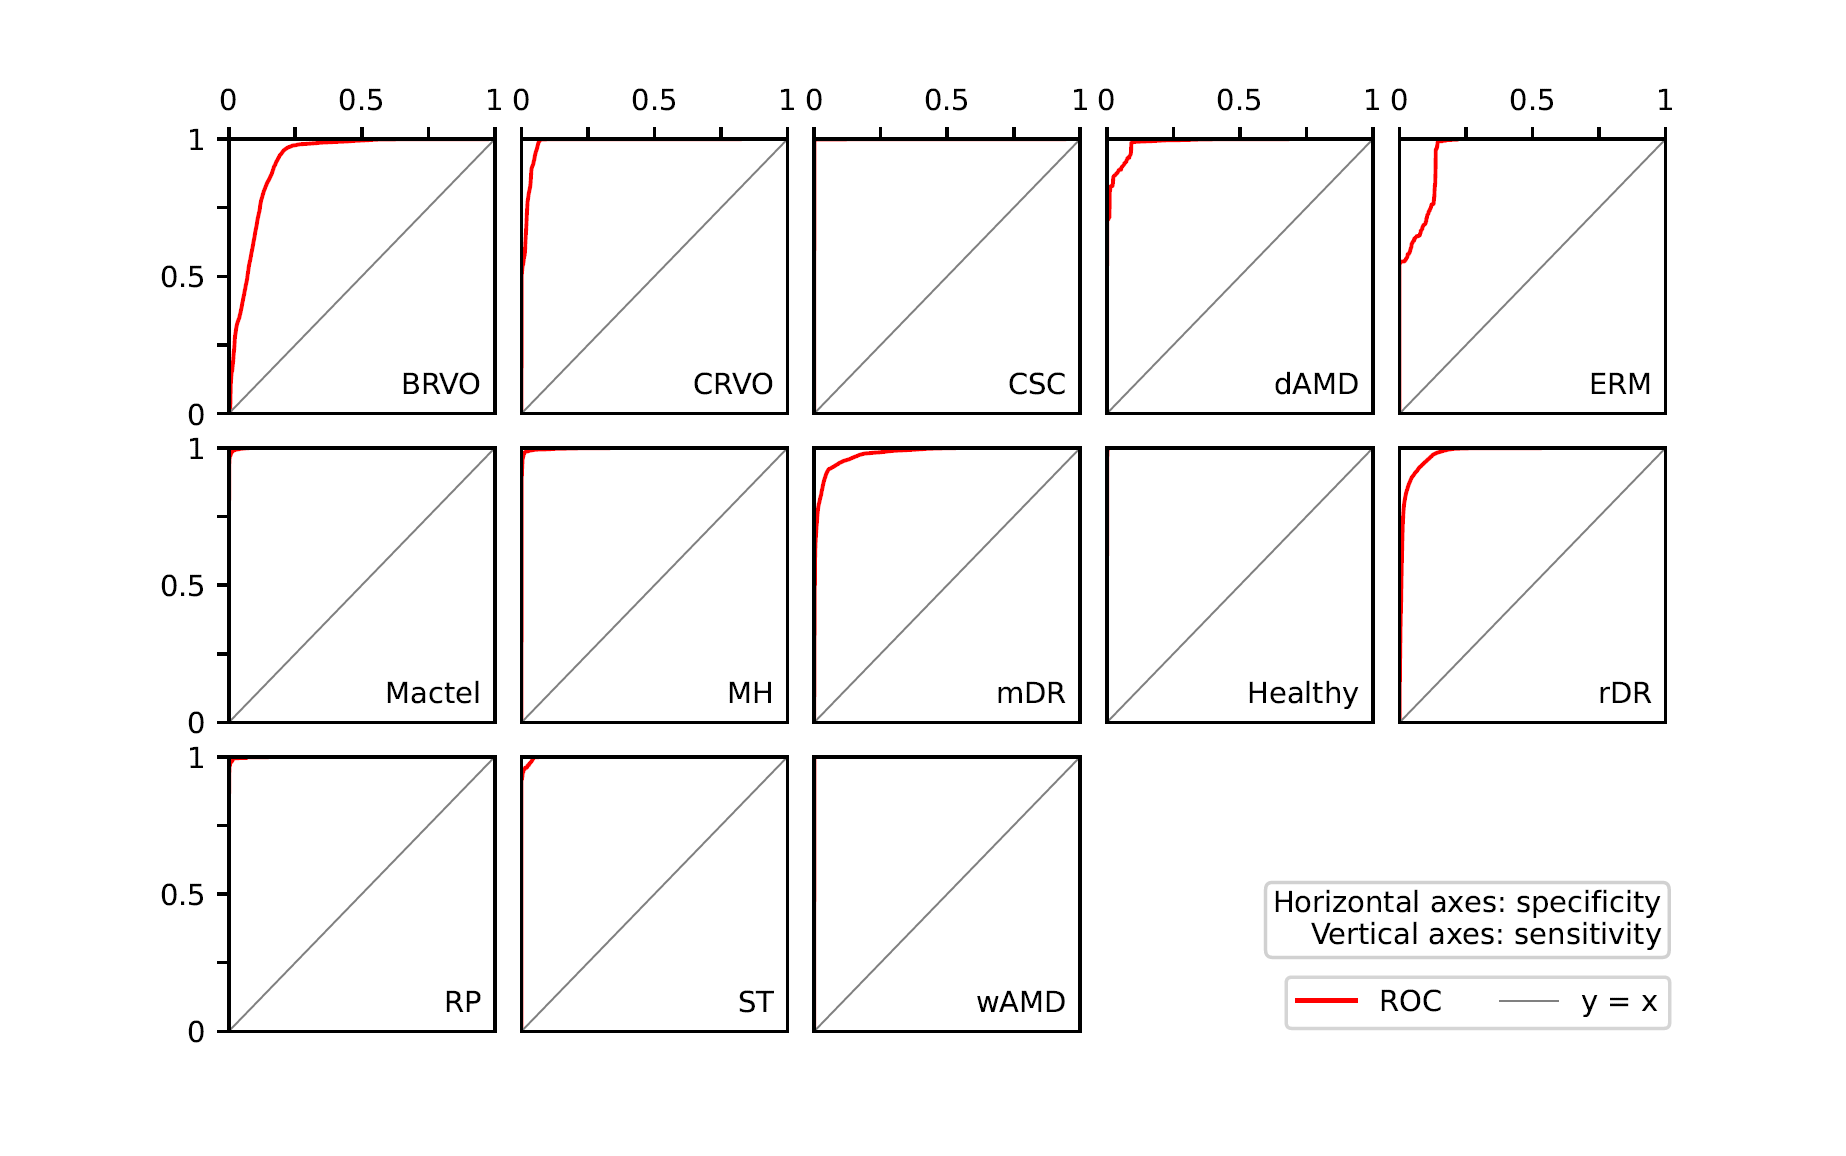
\includegraphics[width=\linewidth]{Figs/diagnosis2_ROC.png}
		\vspace{-0.8cm}
		\caption{阶段D2的ROC曲线}
		\label{fig:D2_ROC}
	\end{figure}
	
	\begin{figure}[H]
		\centering
		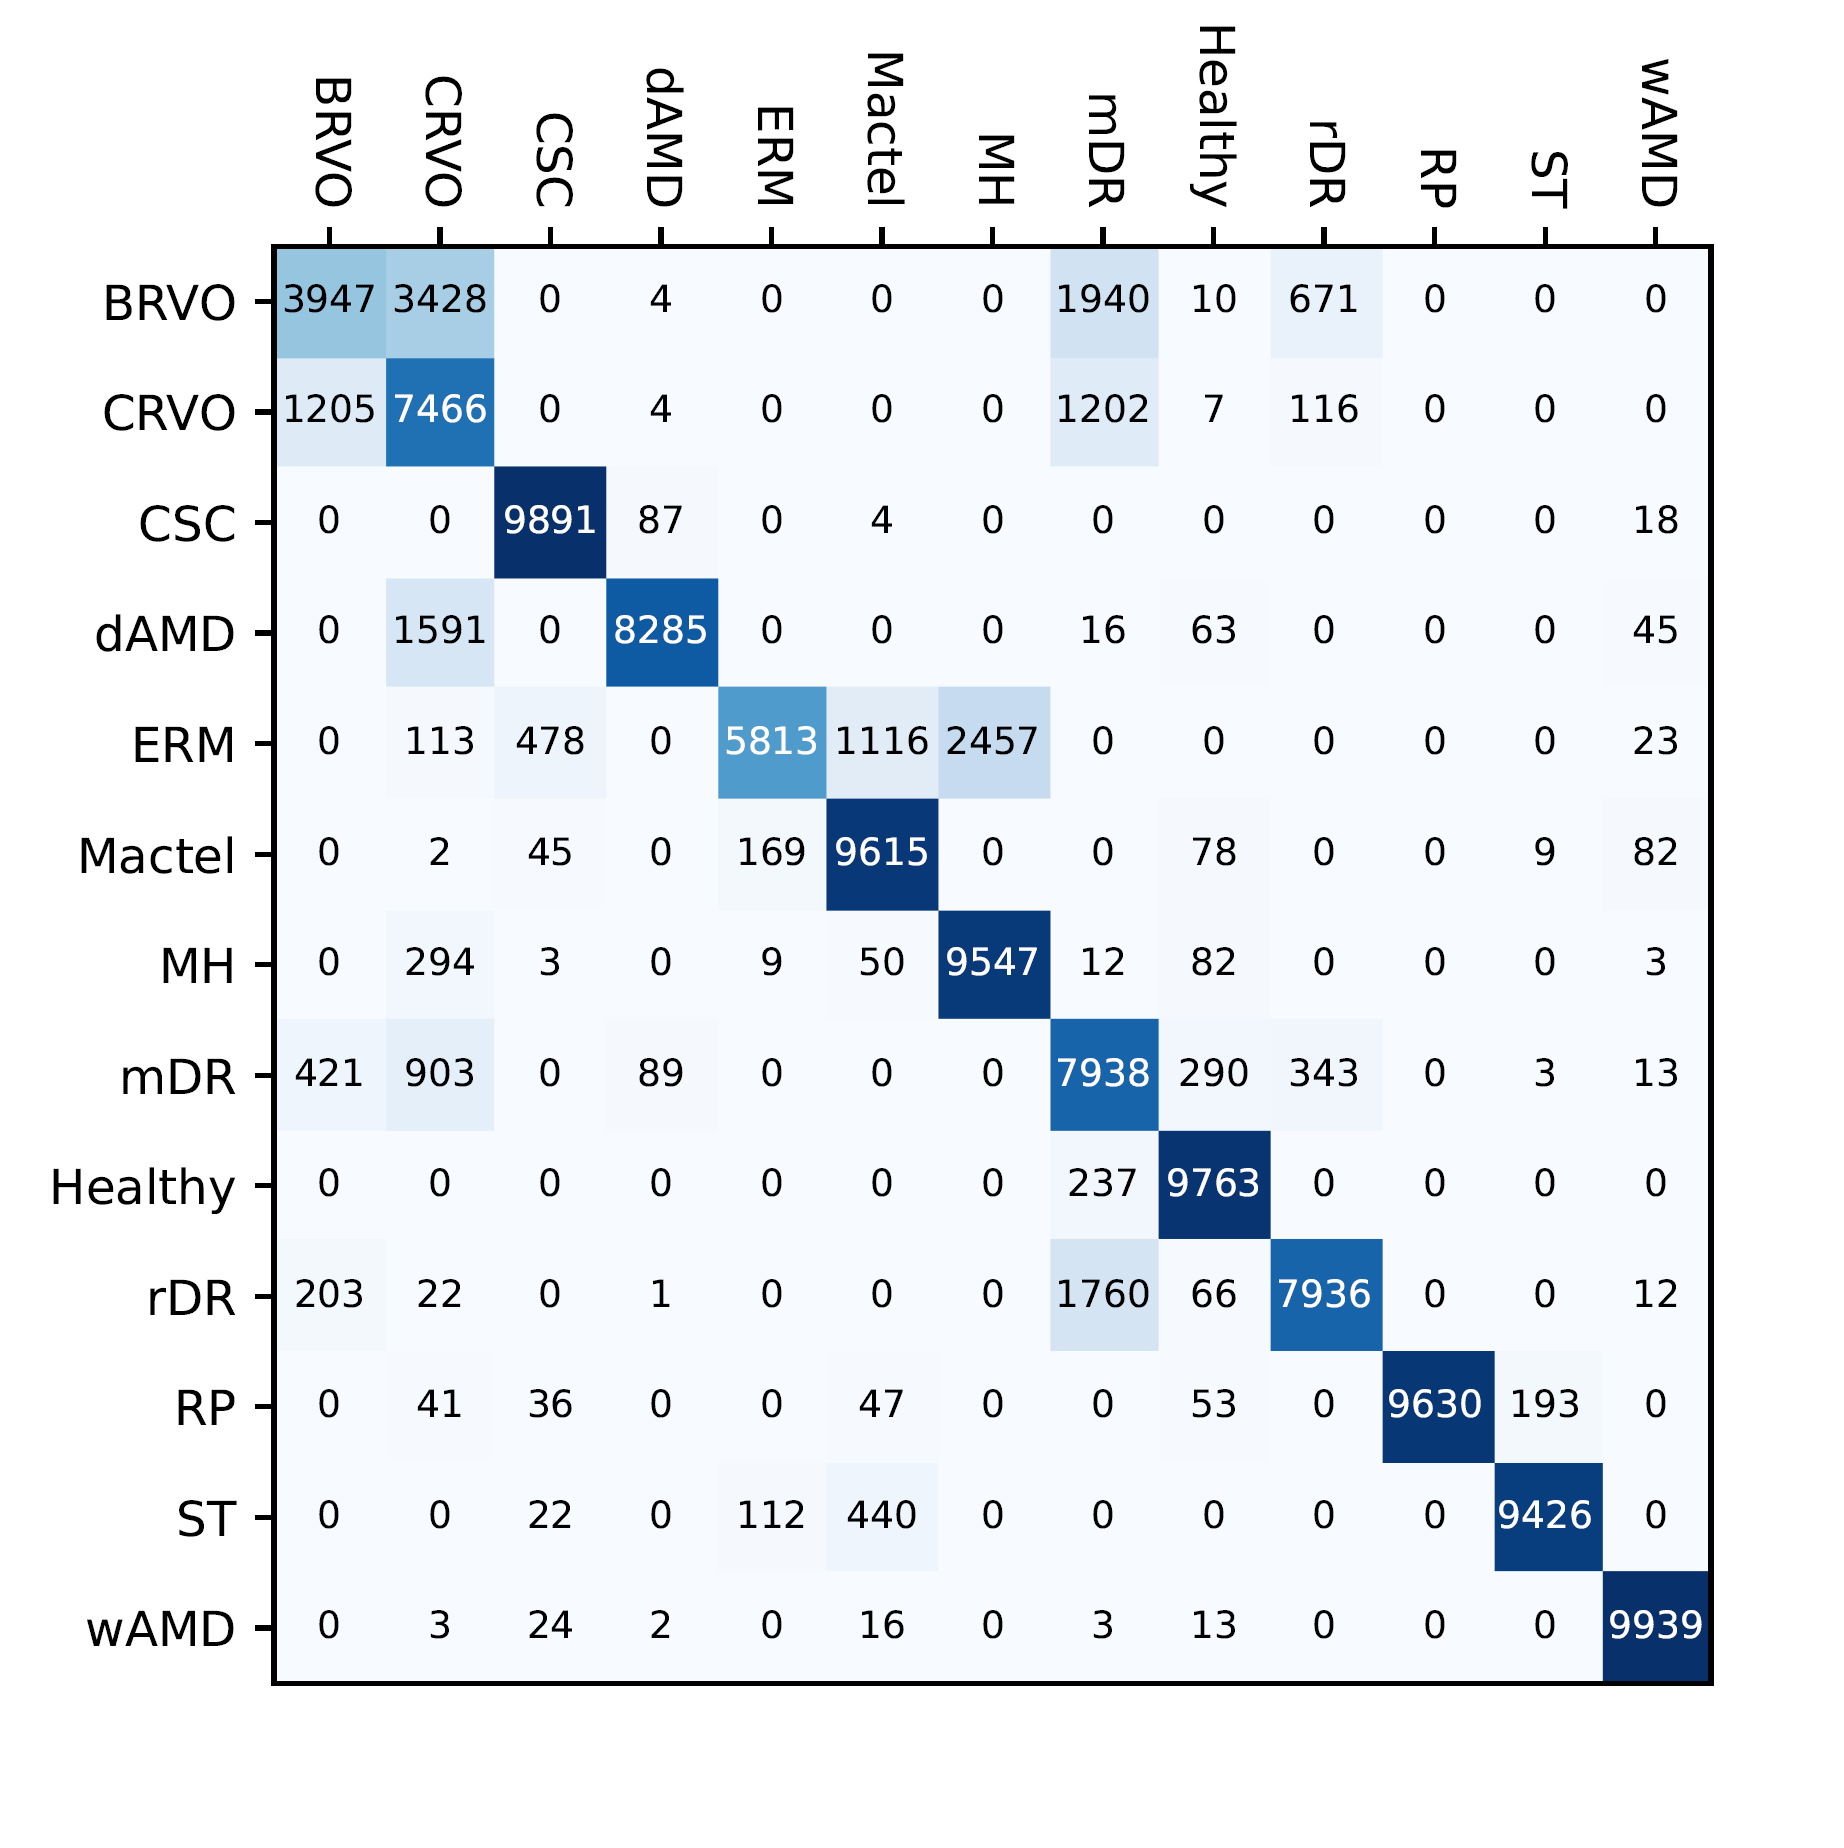
\includegraphics[width=0.7\linewidth]{Figs/diagnosis2_confusion_matrix.png}
		\vspace{-0.8cm}
		\caption{阶段D2的混淆矩阵}
		\label{fig:D2_conf_mat}
	\end{figure}
	
	\begin{figure}[H]
		\centering
		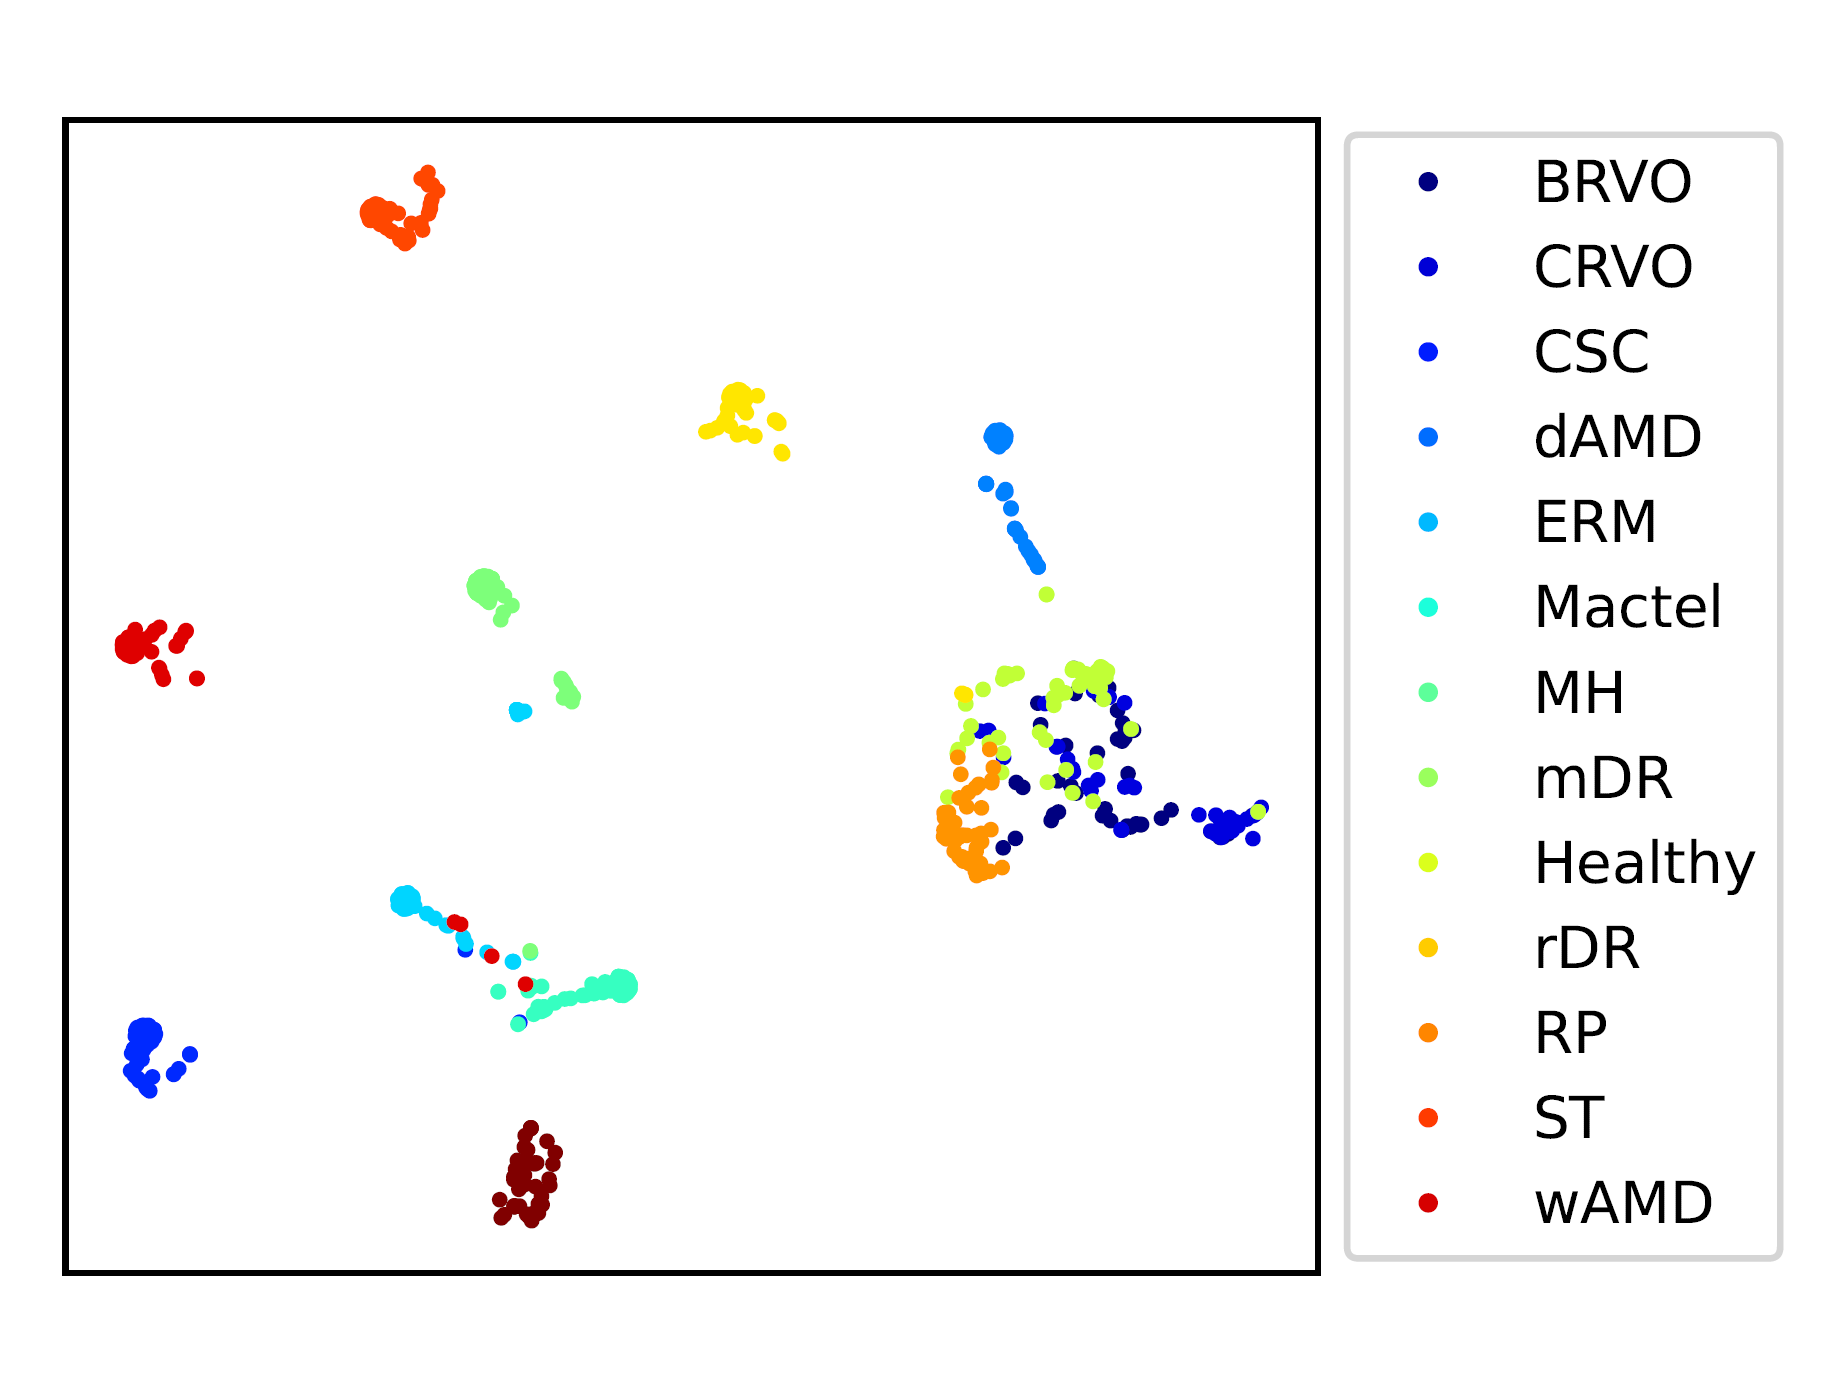
\includegraphics[width=0.65\linewidth]{Figs/diagnosis2_tSNE.png}
		\vspace{-0.3cm}
		\caption{阶段D2的t-SNE图}
		\label{fig:D2_tSNE}
	\end{figure}
	
		\begin{table}[H]
		\centering
		\fontsize{9}{12}\selectfont{
			\caption{阶段D2的测试结果}
			\label{tb:diagnosis_test}
			\pgfplotstabletypeset[
			multicolumn names,
			col sep=comma,
			columns = {Abnormity, Precision, Sensitivity, Specificity, FOne, AUC},
			columns/Abnormity/.style={string type, column name=疾病},
			columns/Precision/.style={string type, column name=精确率},
			columns/Sensitivity/.style={string type, column name=敏感性},
			columns/Specificity/.style={string type, column name=特异性},
			columns/FOne/.style={string type, column name={F1分数}},
			columns/AUC/.style={string type, column name=AUC},
			every head row/.style={before row=\toprule, after row=\midrule},
			every last row/.style={ after row=\bottomrule}
			]{Tables/diagnosis2.csv}}
	\end{table}
	
	\pagebreak
	
	\begin{multicols}{2}
	\section{讨论}
	
	一些研究专注于 OCT 异常分类。例如,\citeauthor{leandro2023oct} 等人的模型在 10770 张图像上训练(大多数图像属于多个类别),能分类 8 种异常,总体准确率在 93\% 到 99\% 之间 \autocite{leandro2023oct}。\citeauthor{li2019deep} 等人的模型在 21357 张图像上训练,能分类 4 种异常,总体准确率为 97.3\% \autocite{li2019deep}。另一些研究专注于眼底异常分类。例如,\citeauthor{Son2023} 等人的模型在 103262 张图像上训练,能分类 15 种异常,平均 AUC 为 0.980 \autocite{Son2023}。相比之下,我们的 OCT 模型在 15632 张图像上训练,能分类 11 种异常,总体准确率不足 80\%;而眼底模型在 1734 张图像上训练,能分类 8 种异常,平均 AUC 为 0.909。事实上,我们的异常模型在性能上并不理想。
	
	我们的数据来自各种在线来源,因此缺乏统一标准。此外,部分数据由我们自己标注,但我们并不具备眼科医生的专业知识。此外,我们的数据量不足,各异常之间的图像数量不平衡。在 OCT 模型中,我们通过使用 Cycle-GAN 部分中和了这种不平衡。然而在眼底模型中,我们只能进行图像变换以生成更多图像,这可能会增加模型的过拟合倾向,使其难以提取正确的特征。此外,如前所述,我们的模型中一张图像上通常存在多个异常,这增加了正确识别特定异常的难度。
	
	\vspace{0.3cm}
	
	在 MAAM 中,诊断模型成功提高了整体性能。也有一些研究使用类似框架。例如,\citeauthor{Son2023} 等人的诊断模型能分类 8 种疾病,平均 AUC 为 0.992 \autocite{Son2023}。相比之下,我们的诊断模型能分类 12 种疾病,平均 AUC 为 0.984,与其他研究接近。
	
	需要注意的是,MAAM 的目标并非识别单一疾病,而是识别所有潜在疾病,这与本文提到的其他研究有所不同。因此,我们引入了共显异常和共显疾病的概念,提升了模型的表现。此外,诊断模型进行了两次特征提取。虽然异常模型的准确率仅在 70\% 到 80\% 之间,但在阶段 D1 提取疾病严重程度的特征后,平均准确率有所提高。并且在阶段 D2 提取疾病特征后,准确率进一步提高,达到了令人满意的水平。这两个阶段提升了异常模型的性能,使疾病特征更加清晰。此外,在训练诊断模型时,我们使用异常-疾病推导标准生成了可靠的标签,即使不涉及眼科医生的专业知识也具备一定的可靠性。
	
	\section{结论}
		
	本研究的主要目标是设计一种新颖的模型并验证其可行性。MAAM 以 OCT 和眼底图像为输入,利用融合机制整合来自不同来源的信息。此外,我们从异常推导疾病,模拟了眼科医生的决策过程。我们还引入了共显异常和共显疾病,提供了更多的参考信息。因此,该模型打破了复杂神经网络的“黑箱”,揭示了更多信息。另一方面,模型仍有改进空间,例如收集更多真实数据、引入眼科医生的专业知识、优化异常-疾病推导标准以及改进诊断模型结构等。
	
	\end{multicols}
	
	\pagebreak
	\phantomsection
	\addcontentsline{toc}{section}{参考文献}
	\newrefcontext[sorting=nyt]
	\begin{multicols}{2}
	\printbibliography
	\end{multicols}
	
	
	\pagebreak
	\section*{附录}
	
	\subsection*{代码}
	
	GitHub 仓库的链接是 \url{https://github.com/SiqiPan2008/MAAM/}。
	
	\subsection*{异常与疾病}
	
	{
		\fontsize{9}{12}\selectfont
		{
			\begin{longtable}{llp{9.5cm}}
				\caption*{OCT异常}
				\label{tb:oct-abnormites}\\
				\toprule
				异常&缩写&描述\\
				\toprule
				
				脉络膜新生血管
				& CNV
				& 脉络膜层中血管异常生长。\\
				
				中心性浆液性脉络膜视网膜病
				& CSC
				& 视网膜下方液体的积聚。\\
				
				糖尿病黄斑水肿
				& DME
				& 与糖尿病视网膜病相关的黄斑液体积聚。\\
				
				脉络膜小疣
				& Drusen
				& 在视网膜色素上皮(RPE)下或RPE与感光细胞层之间积聚的细小外源性物质沉积物。\\
				
				视网膜上膜
				& ERM
				& 在视网膜表面(尤其是黄斑)形成的一层薄薄的纤维组织。\\
				
				视网膜内积液
				& IF
				& 视网膜层内液体的积聚。\\
				
				黄斑裂洞
				& MH
				& 环绕黄斑孔的正常视网膜层的破坏或不连续。\\
				
				黄斑毛细管扩张
				& Mactel
				& 黄斑血管的异常,导致黄斑结构和功能的改变。\\
				
				视网膜色素变性
				& RP
				& 视网膜层变薄,感光细胞层的破坏,视网膜血管的衰退。\\
				
				斯塔格特病
				& ST
				& 视网膜变薄和萎缩,感光细胞层的破坏,视网膜下沉积物的存在。\\
				
				视网膜下积液
				& SF
				& 神经感光视网膜与视网膜色素上皮(RPE)之间液体的积聚。\\
				
				\bottomrule
			\end{longtable}
		}
	}
	
	{
		\fontsize{9}{12}\selectfont
		{
			\begin{longtable}{llp{11.2cm}}
				\caption*{Fundus异常}
				\label{tb:fundus-ab}\\
				\toprule
				异常&缩写&描述\\
				\toprule
				
				棉絮样斑块
				& CWP
				& 白色或近白色病变,形状和边缘不规则,也称为软性渗出物。\\
				
				脉络膜小疣
				& Drusen
				& 小而圆或椭圆形的黄色或白色沉积物。\\
				
				硬性渗出物
				& HE
				& 黄色或黄白色沉积物,边缘清晰,通常分布在血管周围。\\
				
				出血
				& HM
				& 从小点状出血到较大的斑点,鲜红色或深红色,表明氧合血液的存在,随着时间推移,出血颜色可变为深红、橙色或黄色。\\
				
				黄斑裂洞
				& MH
				& 完全厚度的黄斑孔,周围有视网膜下液体的环形带。\\
				
				微动脉瘤
				& MA
				& 视网膜血管中观察到的小血管扩张,表现为视网膜后部散布的小红点。\\

				视网膜色素变性
				& RP
				& 动脉小管变细,视网膜色素变化(低色素或高色素,呈骨刺样或色素聚集)。蜡样盘苍白。\\

				血管异常
				& VA
				& 视网膜血管的扭曲和口径变化。\\
				
				\bottomrule
			\end{longtable}
		}
	}
	
	\pagebreak
	
	{
		\fontsize{9}{12}\selectfont
		{
			\begin{longtable}{cc}
				\caption*{疾病}
				\label{tb:diseases}\\
				\toprule
				疾病&缩写\\
				\toprule
				
				支或半中心视网膜静脉阻塞&BRVO\\
				中心视网膜静脉阻塞&CRVO\\
				中心性浆液性脉络膜病&CSC\\
				干性年龄相关性黄斑变性&dAMD\\
				视网膜上膜&ERM\\
				黄斑毛细血管扩张症&Mactel\\
				黄斑裂洞&MH\\
				轻度糖尿病视网膜病&mDR\\
				可转介糖尿病视网膜病&rDR\\
				视网膜色素变性&RP\\
				斯塔格特病&ST\\
				湿性年龄相关性黄斑变性&wAMD\\
				\bottomrule
			\end{longtable}
		}
	}
	
	\subsection*{图片来源}
	
	\subsubsection*{OCT -- ERM}
	\vspace{0.5cm}
	
	\begin{enumerate}
		\item \nolinkurl{https://qers.com.au/eye-conditions/epiretinal-membrane-erm/}
		
		\item \nolinkurl{https://www.asrs.org/patients/retinal-diseases/19/epiretinal-membranes}
		
		\item \nolinkurl{https://theretinagroup.com/epiretinal-membrane/}
		
		\item \nolinkurl{https://www.istanbulretina.com/en-diseases-epiretinal-membrane.php}
		
		\item \nolinkurl{https://www.mdfoundation.com.au/about-macular-disease/other-macular-conditions/epiretinal-membrane-macular-pucker/}
		
		\item \nolinkurl{https://www.researchgate.net/figure/Grading-of-epiretinal-membrane-ERM-by-spectral-domain-optical-coherence-tomography_fig1_351426760}
		
		\item \nolinkurl{https://www.singhealth.com.sg/patient-care/conditions-treatments/epiretinal-membrane}
		
		\item \nolinkurl{https://www.windycityretina.com/epiretinal-membrane/}
		
		\item \nolinkurl{https://retinacentertx.com/conditions/macular-pucker}
		
		\item \nolinkurl{https://www.rvscny.com/patient-eduction/conditions-we-treat/epiretinal-membrane/}
		
		\item \nolinkurl{https://www.lyneye.co.za/epiretinal-membrane-erm/}
		
		\item \nolinkurl{https://rehmansiddiqui.com/epi-retinal-membrane-erm/}
		
		\item \nolinkurl{https://www.reviewofophthalmology.com/article/when-and-how-to-peel-an-epiretinal-membrane}
		
		\item \nolinkurl{https://www.janigianretina.com/retina-conditions/epiretinal-membrane}
		
		\item \nolinkurl{https://www.researchgate.net/figure/6-months-later-ERM-with-partial-attachment-to-the-retina_fig2_309566437}
		
		\item \nolinkurl{https://www.capefearretina.com/epiretinal-membrane/}
	\end{enumerate}
	
	\subsubsection*{眼底 -- MH}
	\vspace{0.5cm}
	
	\begin{enumerate}
			\item \nolinkurl{https://emedicine.medscape.com/article/1224320-overview}
			
			\item \nolinkurl{https://www.chatswoodeye.com/macular-hole-specialists/}
			
			\item \nolinkurl{https://swretina.com/macular-hole/}
			
			\item \nolinkurl{https://www.ophthalmologyexpertservices.com/blog/2019/macular-hole}
			
			\item \nolinkurl{https://www.researchgate.net/publication/38109568_Bilateral_macular_hole_secondary_to_remote_lightning_strike}
			
			\item \nolinkurl{https://www.researchgate.net/publication/38109568_Bilateral_macular_hole_secondary_to_remote_lightning_strike}
			
			\item \nolinkurl{https://www.reviewofoptometry.com/article/facedown-showdown}
			
			\item \nolinkurl{https://www.gotzaridis.gr/en/conditions/macula/full-thickness-macular-hole}
			
			\item \nolinkurl{https://www.researchgate.net/figure/Fundus-image-of-the-right-eye-of-case-1-a-shows-a-macular-hole-with-associated-retinal_fig1_324657341}
			
			\item \nolinkurl{https://www.girayersoz.com.tr/en/macular-hole/}
			
			\item \nolinkurl{https://www.gotzaridis.gr/en/conditions/macula/full-thickness-macular-hole}
			
			\item \nolinkurl{https://www.gotzaridis.gr/en/conhttps://www.willseye.org/macular-hole/ditions/macula/full-thickness-macular-hole}
			
			\item \nolinkurl{https://www.willseye.org/macular-hole/}
			
			\item \nolinkurl{http://www.oculist.net/downaton502/prof/ebook/duanes/pages/v3/ch031/013f.html}
			
			\item \nolinkurl{https://www.slideshare.net/slideshow/macular-hole-227845841/227845841#11}
			
			\item \nolinkurl{https://www.slideshare.net/slideshow/macular-hole-227845841/227845841#12}
			
			\item \nolinkurl{https://www.jaypeedigital.com/book/9788180616532/chapter/ch7}
			
			\item \nolinkurl{https://emedicine.medscape.com/article/1224320-clinical?form=fpf}
			
			\item \nolinkurl{https://www.jaafarelannanmd.com/macular-hole}
			
			\item \nolinkurl{https://asiaeyecentre.com.sg/eye-conditions/the-ageing-eye/macular-hole/}
			
			\item \nolinkurl{https://retinaandeye.com.au/eye-conditions/full-thickness-macular-holes/}
			
			\item \nolinkurl{https://retinahi.com/interesting-cases/}
			
			\item \nolinkurl{https://imagebank.asrs.org/file/2858/traumatic-macular-hole}
			
			\item \nolinkurl{https://www.semanticscholar.org/paper/Giant-macular-hole-as-an-atypical-consequence-of-a-Blaise-Comhaire/5c9a60375d904323eb5fbcd52b6bd03b735f6951}
			
			\item \nolinkurl{https://webeye.ophth.uiowa.edu/eyeforum/atlas/pages/Macular-hole-commotio-retinae-choroidal-rupture.htm#gsc.tab=0}
			
			
			\item \nolinkurl{https://areaoftalmologica.com/en/terms-of-ophthalmology/macular-hole/}
			
			\item \nolinkurl{https://www.reviewofoptometry.com/article/facedown-showdown}
			
			\item \nolinkurl{https://montanaretinaconsultants.com/portfolio/macular-holes/}
			
			\item \nolinkurl{https://ccteyes.com/2019/09/30/what-is-a-macular-hole-and-how-does-it-affect-your-vision/}
			
			\item \nolinkurl{https://www.backoftheeyemd.com/retina-services/macular-holes/}
			
			\item \nolinkurl{https://www.asrs.org/content/images/cms/image_rib_macularhole_2_2858.jpg/image-full;size$250,194.ImageHandler}
			
			\item \nolinkurl{https://www.asrs.org/content/images/cms/image_rib_macularhole_2_2858.jpg/image-full;size$250,194.ImageHandler}
			
			\item \nolinkurl{https://www.asrs.org/content/images/cms/image_rib_macularhole_2_2858.jpg/image-full;size$250,194.ImageHandler}
			
			\item \nolinkurl{https://webeye.ophth.uiowa.edu/eyeforum/atlas/pages/extrafoveal-macular-hole/emh-1.jpg}
	\end{enumerate}
	
	\subsubsection*{眼底 -- RP}
	\vspace{0.5cm}
		
	\begin{enumerate}
		\item \nolinkurl{https://imagebank.asrs.org/file/93471/retinitis-pigmentosa}
		
		\item \nolinkurl{https://educate.choroida.com/2021/07/05/retinitis-pigmentosa/}
		
		\item \nolinkurl{https://decisionmakerplus.net/dg-post/h35-52-retinitis-pigmentosa/}
		
		\item \nolinkurl{https://basicmedicalkey.com/retinitis-pigmentosa/}
		
		\item \nolinkurl{https://www.news-medical.net/health/What-is-Retinitis-Pigmentosa.aspx}
		
		\item \nolinkurl{https://www.researchgate.net/figure/Fundus-photograph-of-an-individual-affected-with-retinitis-pigmentosa-The-fundus_fig3_40447070}
		
		\item \nolinkurl{https://www.ncbi.nlm.nih.gov/books/NBK11553/figure/ch36clinicalerg.F15/}
		
		\item \nolinkurl{https://www.brainkart.com/article/Retinal-Dystrophies--Retinitis-Pigmentosa_26087/}
		
		\item \nolinkurl{https://entokey.com/retinitis-pigmentosa-and-allied-disorders/}
		
		\item \nolinkurl{https://entokey.com/retinitis-pigmentosa-and-allied-disorders/}
		
		\item \nolinkurl{https://retinography.org/sector-retinitis-pigmentosa/}
		
		\item \nolinkurl{https://retinography.org/sector-retinitis-pigmentosa/}
		
		\item \nolinkurl{https://www.linkedin.com/posts/stevenlevymd_blindness-from-retinitis-pigmentosa-reversed-activity-7047214648877608960-ar4h}
		
		\item \nolinkurl{https://atlas-1-elastic.atlasoph.com/photo.jsf;jsessionid=94EF0B6B067E676E8BCB3F2AD7B9885A?node=6475&locale=en}
		
		\item \nolinkurl{https://dizziness-and-balance.com/disorders/visual/retinopathy/RP.html}
		
		\item \nolinkurl{https://disorders.eyes.arizona.edu/disorders/retinitis-pigmentosa-ar}
		
		\item \nolinkurl{https://disorders.eyes.arizona.edu/disorders/retinitis-pigmentosa-ar}
		
		\item \nolinkurl{https://eyeandear.org/2020/07/a-new-era-in-retinal-research/}
		
		\item \nolinkurl{https://www.ncbi.nlm.nih.gov/books/NBK11553/figure/ch36clinicalerg.F14/}
		
		\item \nolinkurl{https://commons.wikimedia.org/wiki/File:Fundus_of_patient_with_retinitis_pigmentosa,_end_stage.jpg}
		
		\item \nolinkurl{https://healthjade.net/retinitis-pigmentosa/}
		
		\item \nolinkurl{https://www.reviewofoptometry.com/article/night-spots}
		
		\item \nolinkurl{https://www.visualsurgery.com/eye-conditions/retinal-diseases/other-retinal-diseases/retinitis-pigmentosa/}
		
		\item \nolinkurl{https://www.researchgate.net/figure/Fundus-of-an-RP-patient-at-different-stages-a-Image-of-a-normal-healthy-eye-b_fig4_279155571}
		
		\item \nolinkurl{https://www.researchgate.net/figure/Fundus-of-an-RP-patient-at-different-stages-a-Image-of-a-normal-healthy-eye-b_fig4_279155571}
		
		\item \nolinkurl{https://www.researchgate.net/figure/Fundus-of-an-RP-patient-at-different-stages-a-Image-of-a-normal-healthy-eye-b_fig4_279155571}
		
		\item \nolinkurl{https://www.researchgate.net/figure/Fundus-of-an-RP-patient-at-different-stages-a-Image-of-a-normal-healthy-eye-b_fig4_279155571}
		
		\item \nolinkurl{https://emedicine.medscape.com/article/1227488-overview?form=basic}
		
		\item \nolinkurl{https://www.centreforeyehealth.com.au/retinitis-pigmentosa-extract/}
		
		\item \nolinkurl{https://www.centreforeyehealth.com.au/retinitis-pigmentosa-extract/}
		
		\item \nolinkurl{https://www.centreforeyehealth.com.au/retinitis-pigmentosa-extract/}
		
		\item \nolinkurl{https://webvision.med.utah.edu/book/electrophysiology/the-electroretinogram-clinical-applications/}
		
		\item \nolinkurl{https://www.retinarevealed.com/retinitis-pigmentosa-page-34-of-49/}
		
		\item \nolinkurl{http://www.pjo.com.pk/30/2/12.CR%20Sana%20Nadeem%20Corrected.htm}
		
		\item \nolinkurl{http://www.pjo.com.pk/30/2/12.CR%20Sana%20Nadeem%20Corrected.htm}
		
		\item \nolinkurl{https://www.nyp.org/advances/article/ophthalmology/retinitis-pigmentosa-mitigating-retinal-degeneration-with-crispr-technology}
		
		\item \nolinkurl{https://www.ehu.eus/en/-/pacientes-con-retinosis-pigmentaria-en-la-pole}
		
		\item \nolinkurl{https://en.wikipedia.org/wiki/Retinal_degeneration_%28rhodopsin_mutation%29}
		
		\item \nolinkurl{https://imagebank.asrs.org/file/29807/x-linked-retinitis-pigmentosa}
		
		\item \nolinkurl{https://educate.choroida.com/2023/04/07/choroideremia-unveiling-what-you-need-to-know/}
		
		\item \nolinkurl{https://retinography.org/retinitis-pigmentosa-2/}
		
		\item \nolinkurl{https://retinography.org/retinitis-pigmentosa-2/}
		
		\item \nolinkurl{https://retinography.org/retinitis-pigmentosa/}
		
		\item \nolinkurl{https://retinography.org/retinitis-pigmentosa/}
	\end{enumerate}
		
\end{document}